%
% Thesis - Main
% Jack McLean
% School of Computer Science
% University of St Andrews, Scotland, UK
% 2021
%

\documentclass{stacsthesis}

%
% Packages
%
\usepackage[english]{babel}
\usepackage{graphicx}
\usepackage{soul}
\usepackage{color}
\usepackage{hyperref}
\usepackage{tabulary}
\usepackage{booktabs}
\usepackage{listings}
\usepackage{enumitem}
\usepackage{pifont}
\usepackage[nointegrals]{wasysym}
\usepackage{amsmath}
\usepackage{syntax}
\usepackage{textcomp}
\usepackage[font=small,labelfont=bf,skip=16pt]{caption}
\usepackage{hyperref}
\usepackage{natbib}
\usepackage{float}
\usepackage{placeins}
\usepackage{booktabs,caption,fixltx2e}
\usepackage[flushleft]{threeparttable}
\usepackage[margin=1in]{geometry}
\usepackage[utf8]{inputenc}
\usepackage[toc]{glossaries}
\usepackage{hyperref}


\makeglossaries
\loadglsentries{glossary}

%
% Compiler warnings
%
\hfuzz=10pt 
\vfuzz=10pt
\hbadness=10000
\vbadness=10000

%
% Configure code listings
%
\lstset {
	language=Java,
	basicstyle=\footnotesize\ttfamily\singlespacing,
	showstringspaces=false,
	keywordstyle=\color[RGB]{0, 0, 240},
	stringstyle=\color[RGB]{240, 0, 0},
	commentstyle=\color[RGB]{0, 144, 0},
	numberstyle=\tiny,
	basewidth=0.54em,
	tabsize=2,
	captionpos=b,
	frame=tb,
	framesep=10pt,
	aboveskip=8pt,
	belowskip=0pt,
	abovecaptionskip = 16pt,
	breakindent=24pt,
	breaklines=true,
	numberbychapter=true
}

%
% Console output
%
\lstdefinestyle{console} {
	language=bash,
	basicstyle=\footnotesize\ttfamily\singlespacing,
	backgroundcolor=\color[RGB]{248, 247, 242},
	upquote=true,
	frame=single,
	framerule=0pt,
	breakindent=0pt,
	breaklines=true,
	aboveskip=0pt,
	belowskip=4pt,
	xleftmargin=10pt,
	xrightmargin=10pt
}

%
% Inline coding listing commands
%
\def\javacode{\lstinline[basicstyle=\bfseries\ttfamily,basewidth=0.48em,language=Java]}

%
% Custom commands
%

%
% Configure caption and sub-caption styles
%
\newsubfloat{figure}
\captionnamefont{\bfseries\small}
\captiontitlefont{\small}
\subcaptionlabelfont{\bfseries\footnotesize}
\subcaptionfont{\footnotesize}

%
% Customise titles names
%
\bibtitle{References}

%
% Customise toc
%
\maxtocdepth{subsection}

%
% Chapter and page style
%
\pagestyle{stacs-pg}

%
% Control word hyphenation
%
\hyphenpenalty=512
\tolerance=1024
\emergencystretch=4pt
\hyphenation{
	arti-ficial com-puter imple-ment imple-men-tation imple-men-ting frame-work
	Java
}

%
% Title page
%
\begin{document}
\hypersetup{pageanchor=false}
\title{\textbf{Managing Labs}\\Developing Lab Management Software for the New Normal}
\author{Jack McLean \textbf{190025023}}
\supervisor{Ruth Letham}
\school{School of Computer Science}
\degree{MSc Computing \& Information Technology}
\submittextA{This thesis is submitted in partial fulfilment for the degree of}
\submittextB{at the University of St Andrews, School of Computer Science}
\submitdate{August 2021}
\maketitle

%
% Prologue
%
\begin{abstract}
Abstract goes here.

general todos:
\begin{itemize}
    \item figure captions
    \item blank page issues!
    \item get a better referencing style
    \item depth of sub sections in TOC correct or should it display subsubsections
\end{itemize}

\end{abstract}

\begin{acknowledgement}
Acknowledgements go here.
\end{acknowledgement}
%
% Thesis - Declaration
% Jack McLean
% School of Computer Science
% University of St Andrews, Scotland, UK
% 2014
%

\begin{declaration}
\subsection*{Candidate's Declarations}
I, Jack McLean, hereby certify that this thesis, which is approximately \hl{<word-count>} words in length, has been written by me, that it is the record of work carried out by me and that it has not been submitted in any previous application for a higher degree.

I was admitted as a student for the degree of Master of Science in September, 2020; the final research part of these studies, for which this dissertation is presented, was carried out in the University of St.\ Andrews between May 2021 and August 2021.
\vspace{24pt}

Date:
\vspace{16pt}

Signature of candidate:
\vspace{48pt}


\subsection*{Supervisor's Declaration}
I hereby certify that the candidate has fulfilled the conditions of the Resolution and Regulations appropriate for the degree of Master of Science in the University of St.\ Andrews and that the candidate is qualified to submit this thesis in application for that degree.
\vspace{24pt}

Date:
\vspace{16pt}

Signature of supervisor:
\end{declaration}
%
% Thesis - Permissions
% Jack McLean
% School of Computer Science
% University of St Andrews, Scotland, UK
% 2014
%


\begin{permission}
In submitting this thesis to the University of St Andrews I understand that I am giving permission for it to be made available for use in accordance with the regulations of the University Library for the time being in force, subject to any copyright vested in the work not being affected thereby. I also understand that the title and the abstract will be published, and that a copy of the work may be made and supplied to any bona fide library or research worker, that my thesis will be electronically accessible for personal or research use unless exempt by award of an embargo as requested below, and that the library has the right to migrate my thesis into new electronic forms as required to ensure continued access to the thesis. I have obtained any third-party copyright permissions that may be required in order to allow such access and migration, or have requested the appropriate embargo below.

The following is an agreed request by candidate and supervisor regarding the electronic publication of this thesis:

\begin{indentpara}
\emph{Access to printed copy and electronic publication of thesis through the University of St Andrews.}
\end{indentpara}

\vspace{24pt}

Date: \today
\vspace{16pt}

Signature of candidate:
\vspace{48pt}

Signature of supervisor:
\end{permission}


%
% Tables of contents/figures/tables
%
\cleardoublepage
\hypersetup{pageanchor=true}
\pagenumbering{roman}
\tableofcontents
\newpage\listoffigures
\newpage\listoftables
\newpage\lstlistoflistings

%
% Mainmatter properties
%
\mainmatter
\onehalfspacing
\pagenumbering{arabic}
\setlength{\parskip}{3mm}
\setlength{\parindent}{0mm}
\setlist[enumerate]{leftmargin=*,labelsep=0.8em,topsep=0em,parsep=0.6em}
\setlist[itemize]{leftmargin=*,labelsep=1.0em,topsep=0em,parsep=0.6em,label=\normalsize\textbullet}
\newenvironment{itemize*}			% Itemising environment for single-lined items
	{\begin{itemize}					% Interline spacing has been adjusted in this case to
    		\setlength{\itemsep}{0.016em}}	% make the itemised text look more consistent with the rest
     	{\end{itemize}}


%
% Content
%
\chapter{Introduction}

%The School of Computer Science at the University of St.\ Andrews has historically run lab sessions for early years students, offering them support in developing their practical programming skills. The school traditionally operated these labs using a ‘hands-up’ system to organise in-class support, however the school's relatively rapid growth in class size means that this method is becoming less efficient. The global pandemic has further accelerated the need for an alternative support system, since the in-person labs replacement with online sessions meant that the traditional system was not possible. 

In the early 2000s, the University of St.\ Andrews' School of Computer Science had a class size of approximately 30 students. It has had a relatively rapid expansion in recent years, with class size of up to 200 students. Although the student to staff ratio in manned computer laboratory sessions has remained fairly consistent throughout the years, the logistics of class management became more difficult. This increasing difficulty has been increasing educators awareness of the need for an alternative solution.

As lockdown measures were introduced in the wake of the global pandemic, the University was forced to move to online learning and the need for an alternative to in-person labs became immediate. Completely remote online teaching is a novel experience for the University, presenting many challenges. The School developed a system for managing online labs using Microsoft Teams \cite{teams}, adapting it in an ad hoc manner to improve the flow and features by integrating with additional systems such as Sharepoint Lists \cite{lists}, Forms \cite{forms} and Power Automate \cite{pauto}. The current system meets the basic needs for managing online labs, however, it lacks more sophisticated lab management facilities, such as gathering statistical data as well as searching and recommending solutions to posted problems.   
The School of Computer Science requires a system for managing labs that meets its specific needs. The system should be suitable for in-person, remote and dual delivery. It should enable class demonstrators to assist in the resolution of problems students have, should enable lab leads to review labs and address some of the specific nuances that the domain requires - for example addressing the lab opening times. A single application should meet these needs so that the system is easy to use, adapt and maintain.

There are some existing categories of application which could meet the above needs. A small number of classroom management tools exist in the form of queue management systems. Another, much more common, type of application are incident management tools - often used for tracking and logging IT incidents and problems. Both types of application shall be considered and evaluated in order to gain insight into their suitability.

This dissertation begins by outlining the objectives for the project - the development of `codeHelper', the online lab facilitation tool. The second chapter contains a literature review concerning coding in online learning, after which is a discussion about the current system and the existing categories of application discussed above. The third chapter outlines the requirements of the project. The fourth chapter discusses existing applications which were analysed that could fit the problem domain. The fifth chapter discusses the software engineering process which was followed to develop the codeHelper application. The sixth chapter is concerned with design - discussing the more major and interesting design choices for the system architecture, interface and database. The seventh chapter covers the implementation of the system, discussing the major decisions taken. The eighth briefly discusses the types, approach to and implementation of testing throughout the project. The ninth chapter is an evaluation of the developed system, including a discussion of the evaluation participant experiment that was carried out as well as a comparison between codeHelper and the other systems discussed in chapters \ref{chap:context} and \ref{chap:existingtools}. The tenth, and final, chapter concludes the dissertation by discussing limitations and possible future work.

\newpage
\section{Objectives}

The overall goal of this project is to create a custom system for the School that can be used to manage students' requests for practical programming assistance, both in virtual and physical lab sessions. Objectives for the project, as well as which were completed, are listed below. 

The main contribution of the dissertation to the field was providing a tool that allows staff to effectively manage the provision of one-to-one assistance for both in-person and remote settings. Although the system is not production ready, it provides proof of concept that a bespoke system for managing labs is both possible and would make the process more efficient.

\subsection{Primary}
\begin{itemize}
    \item [PO1] \textit{Completed} - Investigate and evaluate existing methods of managing labs, identifying weak points.
    \item [PO2] \textit{Completed} - Undertake established software engineering techniques to plan and design the lab management system.
    \item [] Create a system on which:
    \begin{itemize}
        \item [PO3.1] \textit{Completed} - Students are able to create `tickets' to request help from class demonstrators through a web interface.
        \item [PO3.2] \textit{Completed} - Class demonstrators are able to assign, resolve, close and communicate about `tickets'.
        \item [PO3.3] \textit{Completed} - Staff are able to view statistics and summaries of activity - for example which `tickets' were resolved by which demonstrator, the average time of resolution and the amount of time the `tickets' were open.
    \end{itemize}
    \item [PO4] \textit{Completed} - Evaluate a prototype of the system using volunteer sets of class demonstrators, then complete a final evaluation without external parties. 
    
\end{itemize}

\subsection{Secondary}
\begin{itemize}
    \item [SO1] \textit{Completed} - Implement graphical representation of statistics and summaries generated by the system.
    \item [SO2] \textit{Completed} - Implement a live text chat element on each ticket, allowing interaction between the demonstrator and student.
\end{itemize}

\subsection{Tertiary}
\begin{itemize}
    \item [TO1] Implement authentication on the system using the Shibboleth single sign-on system used by the University of St. Andrews.
    \item [TO2] \textit{Completed} - Implement a method to allow students and class demonstrators to communicate by video chat. 
    \item [T03] Create a user interface recommending anonymised `tickets' to students that may be similar to the their request.
    \item [T04] \textit{Completed} - Implement a screen sharing feature on each ticket, allowing interaction between the demonstrator and student.
    \item [T05] \textit{Partially Completed} - Optimise the system for use on mobile devices. 
\end{itemize}




 

\chapter{Context Survey}
\section{Context}

The University of St.\ Andrews' School of Computer Science originally had a class size of approximately 30 students. It has had a relatively rapid expansion, with class size of over 200 students. Although the student to staff ratio has remained fairly consistent (somewhere between 30 and 20 to 1) throughout the years, the logistics of class management became more difficult. Educators have becoming aware of this increasing need for an alternative solution.

Moving to online learning in the wake of the global pandemic, the need for an alternative became immediate. The school developed a system for managing online labs using Microsoft Teams \cite{teams}, adapting it in a fairly expedient manner. The current system meets the basic needs for managing online labs, however is lacking in a few key areas.  

The School of Computer Science requires a system for managing labs that meets its specific needs. The system should enable class demonstrators to assist in the resolution of problems students have, should enable lab leads to review labs and address some of the specific nuances that the domain requires - for example addressing the lab opening times. A single application should meet these needs so that the system is easy to use, adapt and maintain.

There are some existing categories of application which could meet the above needs. A small number of classroom management tools exist. Another, much more common, type of application are incident management tools - often used for tracking and logging IT incidents and problems. Both types of application shall be considered and evaluated in order to gain insight into their suitability.
 
This section shall discuss and review two common examples of these types of application, as well as the current system used by the school.

\section{Current System}

The current system for managing online lab sessions was developed and adapted at short notice due to the global pandemic. The initial solution was to create a `CS1000 Labs' team on Microsoft Teams \cite{teams}, the University's standard collaboration tool for online learning, and manage the lab sessions by posting announcements when labs opened. Students were then able to post new conversations under these announcements, which prompted them to tag the class demonstrators, and briefly summarising their issue and provide module code and practical number associated with their issue.

TODO: power automate flows owned by system admin, in control of them/nobody else can access them,
TODO collaboration students lost, cheating
TODO: maintenance locations, complicated sharepoint/automate

\FloatBarrier
\begin{figure}[H]
  \centering
  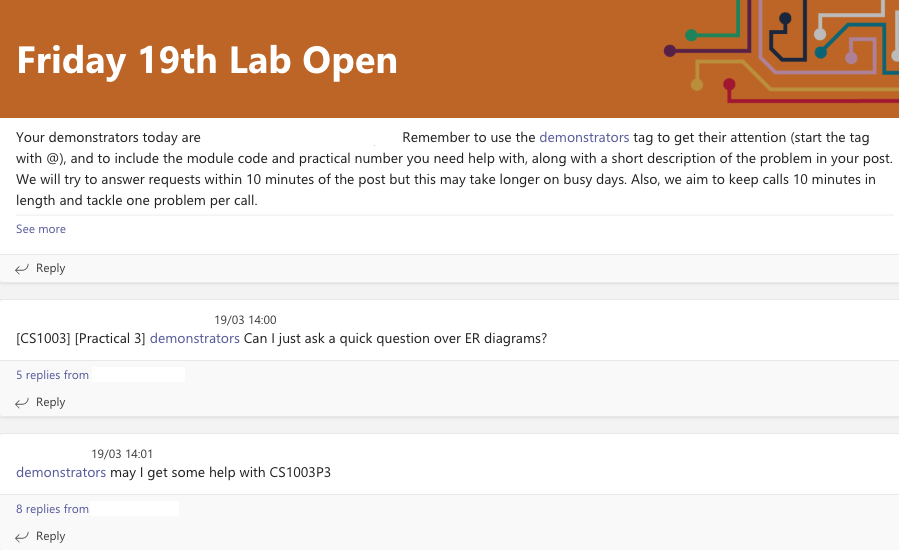
\includegraphics[width=\textwidth]{2context/images/teams1.png}
  \caption{An example of the first iteration process of managing online labs.}
\end{figure}

The second, and current, iteration of the current system uses a form input. This is accessed using a `Request Form' tab in the Microsoft Teams \cite{teams} CS1000 Labs team. 

\FloatBarrier
\begin{figure}[H]
  \centering
  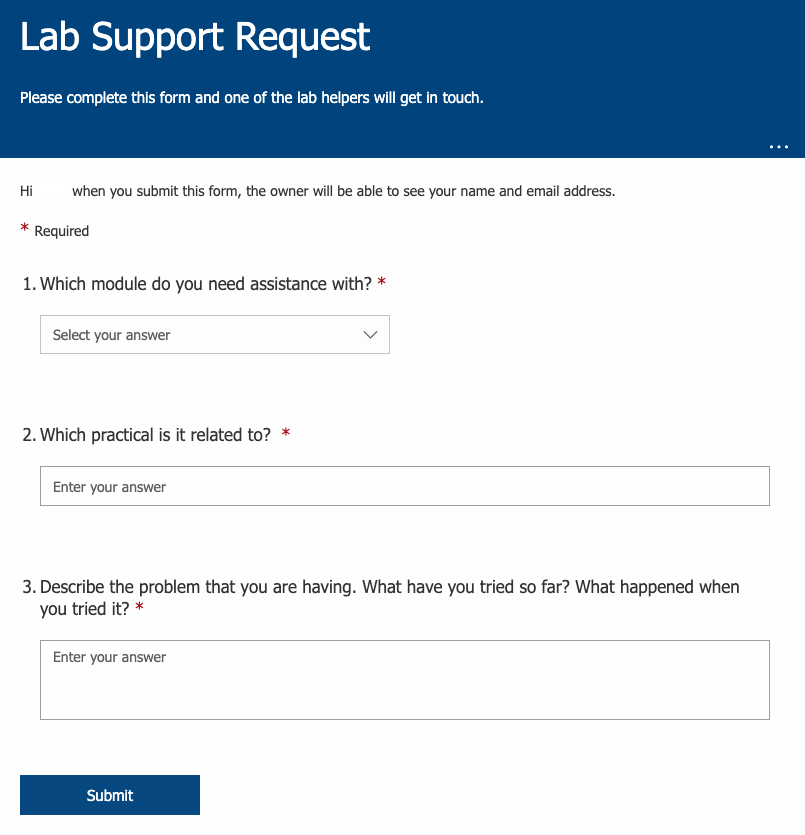
\includegraphics[width=0.85\textwidth]{2context/images/teams2a.png}
  \caption{The request form from the second iteration process of managing online labs.}
\end{figure}

The form uses Power Automate \cite{pauto} to post on a private demonstrator team channel (used only to create a notification for class demonstrators) and add the form data to a Microsoft List \cite{lists}.

\FloatBarrier
\begin{figure}[H]
  \centering
  
\includegraphics[width=0.6\textwidth]{2context/images/teams2b.png}
  \caption{The format of posts on the private demonstrator channel used to create notifications.}
\end{figure}

On this real-time collaborative spreadsheet, class demonstrators can assign themselves to students' requests before they make contact with the student through Microsoft Teams \cite{teams} or email. 

TODO notes:
\begin{itemize}
  \item communication in video or text (depending on issue complexity) but both on teams
\end{itemize}

\FloatBarrier
\begin{figure}[H]
  \centering
  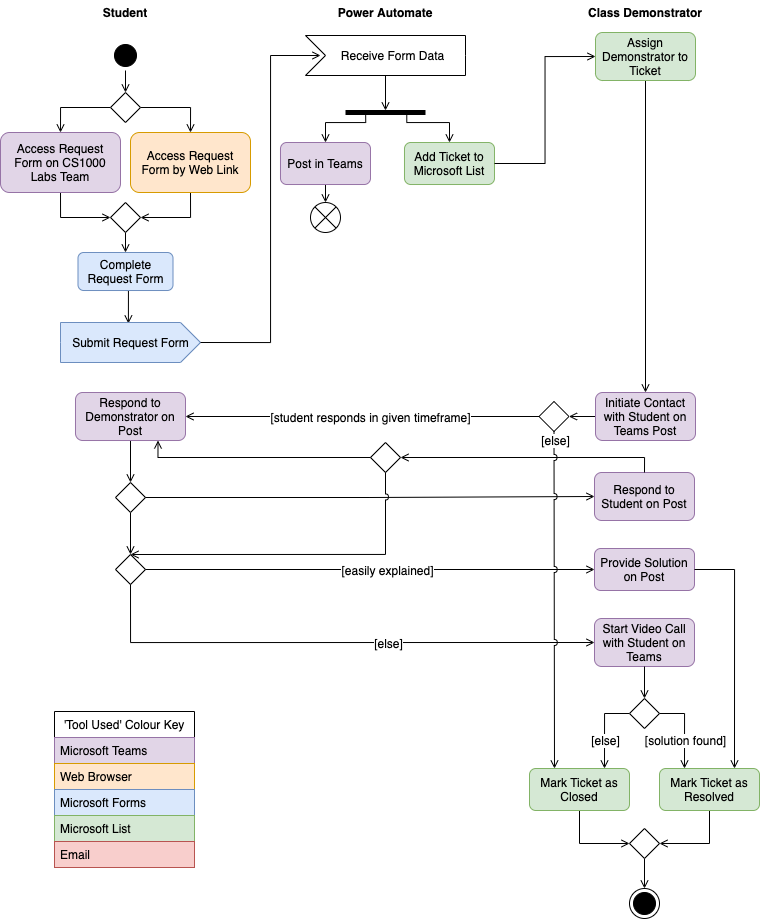
\includegraphics[width=\textwidth]{2context/images/activityRevised.png}
  \caption{Activity diagram for existing method of managing student online lab request.}
\end{figure}

\newpage
\section{Classroom Management Tools}

ClassroomQ is a good example of existing classroom management tools. It offers a very simple system, where teachers can create a classroom which students can join, type a message and hit an `Assistance Needed' button to join the queue of students who need help. The basic process is shown below.

Firstly, the teachers start a classroom session.

\FloatBarrier
\begin{figure}[H]
  \centering
  
\includegraphics[width=0.5\textwidth]{2context/images/cq1.png}
  \caption{Teacher's screen when a class has not been started.}
\end{figure}

The classroom is created, showing the class code which students can use to join.

\FloatBarrier
\begin{figure}[H]
  \centering
  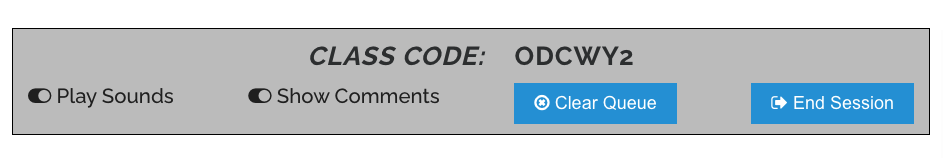
\includegraphics[width=0.75\textwidth]{2context/images/cq2.png}
  \caption{Real time classroom queue, showing class join code and current requests.}
\end{figure}

Students join by entering their name and class code.

\FloatBarrier
\begin{figure}[H]
  \centering
  
\includegraphics[width=0.5\textwidth]{2context/images/cq3.png}
  \caption{Student join page, showing sample class code and name.}
\end{figure}

Below is the image shown to students once they have joined the class. From this page they are able to type details of their problem in the comment section and then click the `Assistance Needed' button to join the queue.

\FloatBarrier
\begin{figure}[H]
  \centering
  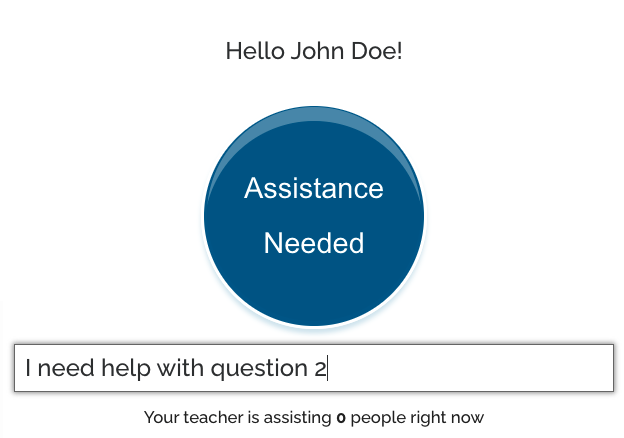
\includegraphics[width=0.5\textwidth]{2context/images/cq4.png}
  \caption{Student help request page.}
\end{figure}

Once the student has joined the queue, they are taken to the page below. This allows them to cancel their request as well as providing real time information about their position in the queue.

\FloatBarrier
\begin{figure}[H]
  \centering
  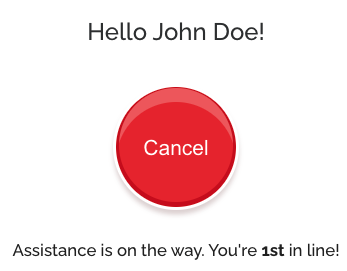
\includegraphics[width=0.5\textwidth]{2context/images/cq5.png}
  \caption{Student page after posting help request.}
\end{figure}

The teacher is then able to see an ordered view of the student's requests in on the class page.

\FloatBarrier
\begin{figure}[H]
  \centering
  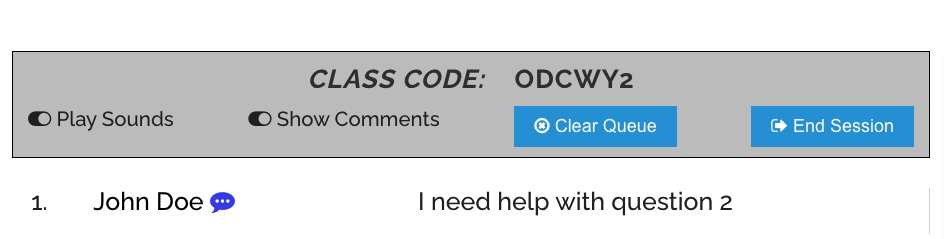
\includegraphics[width=0.75\textwidth]{2context/images/cq6.png}
  \caption{Teacher's class page view after the request has been posted.}
\end{figure}

\newpage
\section{Incident Management Tools}

Spiceworks Cloud Help Desk is a good example of existing incident management tools. It is a free to use, cloud-based help desk that is used by IT professionals. Traditionally, the system is used to track and manage IT issues in order to provide IT support, however the system could also be used to track and manage requests for help in our lab management domain. The basic process is shown below.

Firstly, students would access a link to the help portal and enter their email address.

\FloatBarrier
\begin{figure}[H]
  \centering
  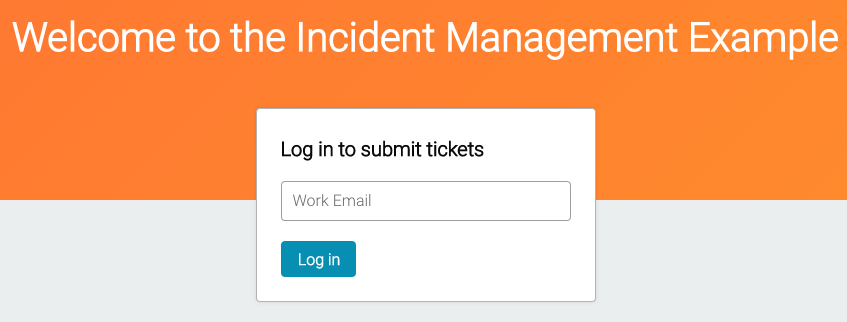
\includegraphics[width=0.5\textwidth]{2context/images/SWportalLogin.png}
  \caption{Login screen from portal link.}
\end{figure}

The student would then, if authorised, receive an email link to login to the portal. This would take them to the following form.

\FloatBarrier
\begin{figure}[H]
  \centering
  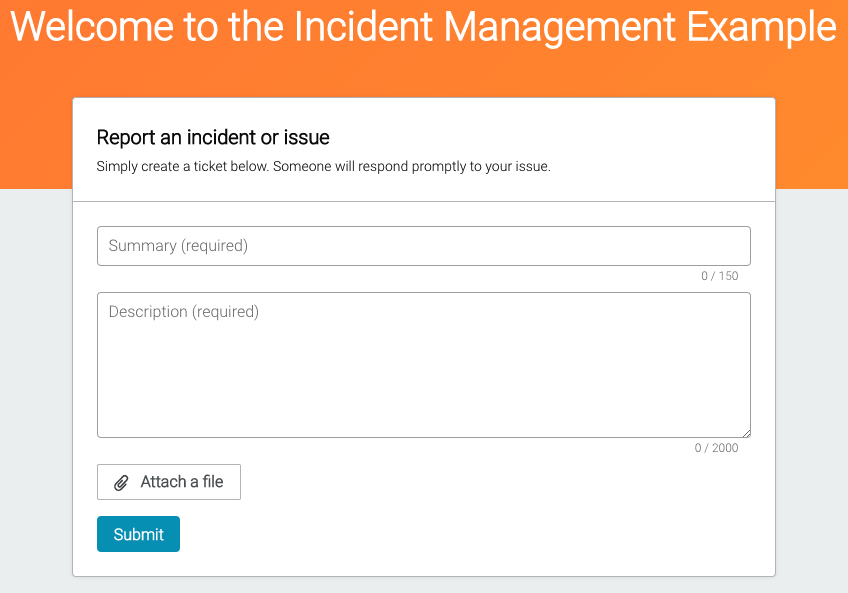
\includegraphics[width=0.65\textwidth]{2context/images/SWpostTicket.png}
  \caption{Ticket posting form, reached after login.}
\end{figure}

The ticket would then appear on the class demonstrator help desk.

\FloatBarrier
\begin{figure}[H]
  \centering
  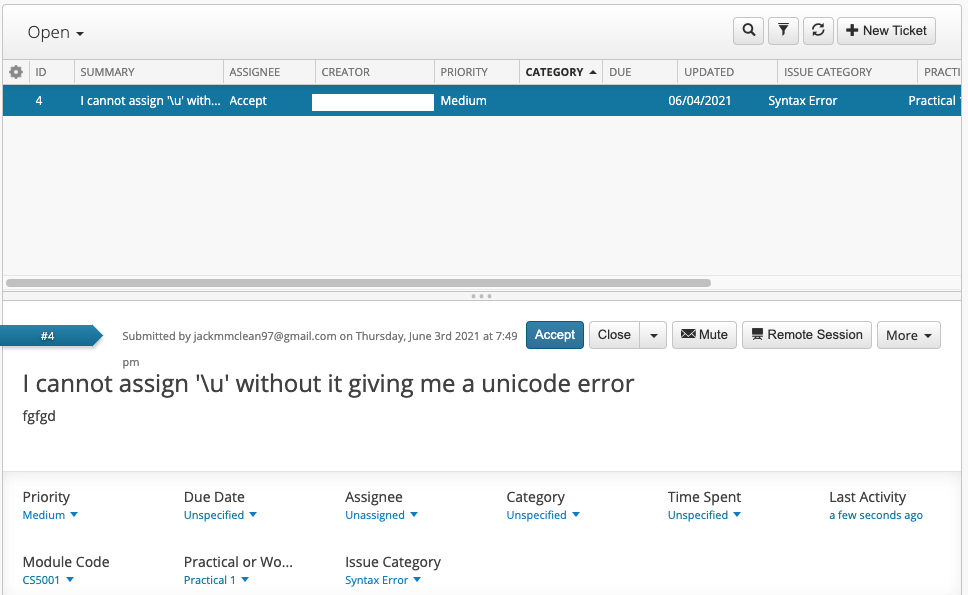
\includegraphics[width=0.85\textwidth]{2context/images/SWticketPage.png}
  \caption{The help desk ticket page, accessible to class demonstrators.}
\end{figure}

Class demonstrators are then able to respond to the ticket on Spiceworks, notifying the user by email, and initiate a video call on a different service if necessary. The demonstrator can then close the ticket when complete.


\chapter{Requirements Specification}
\label{chap:req}
In this chapter we shall outline the system requirements. The first section shows a \gls{uml} use case diagram, used to explore and convey uses of the system in order to help derive requirements. The second section defines the requirements outright.

\section{Use Case}

\subsection{Use Case Diagram}

\begin{figure}[H]
    \centering
    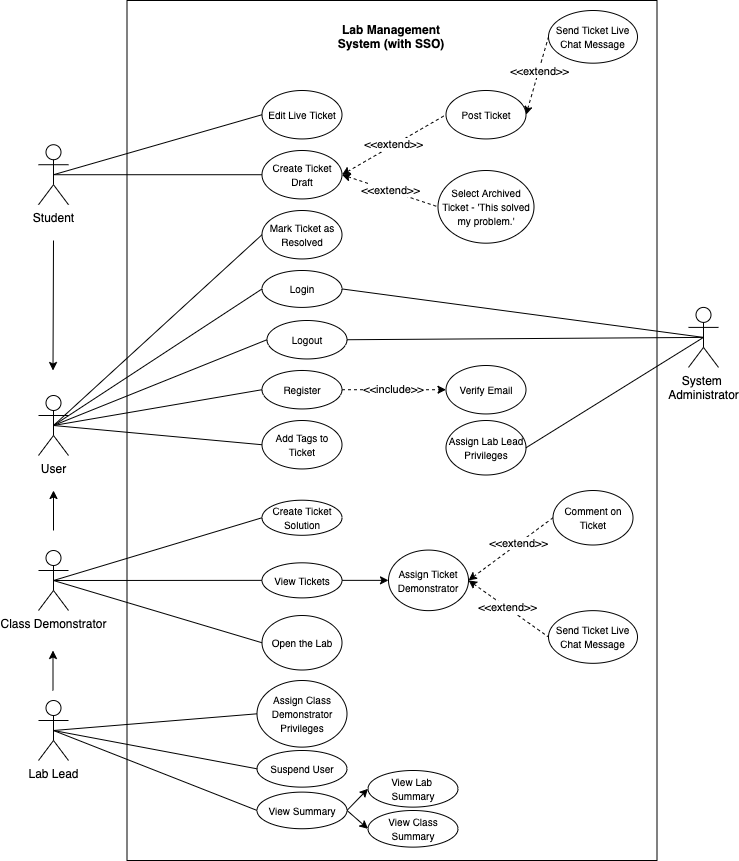
\includegraphics[width=\textwidth]{3requirements/images/useCase.png}
    \caption{Use case diagram for lab management system.}
    \label{fig:useCase}
\end{figure}

\subsection{Use Case Specifications}

\subsection*{`Create Ticket Draft' Use Case Specification}
\begin{table}[H]
\centering
 \begin{tabular}{p{0.27\linewidth}  p{0.67\linewidth}}
 \textbf{Use case name} & \textbf{Post Ticket}  \\
 Use case ID & 1\\
 Brief Description & A student creates a ticket draft on the system.\\
 Preconditions & The student is a registered and verified, the lab is open.\\
 Primary actors & Student. \\
 Secondary actors & \textbf{None.} \\
 Successful end condition & A new live ticket is posted onto the system for class demonstrators to view. \\
 Failed end condition & The ticket listing is rejected. \\
 Main flow & Steps:\\
 & 1. The use case starts when a student tries to visit the `post a ticket' page.\\
 & 2. The system checks that the user is logged in as a registered, verified account with student role privileges. \\
 & 3. The `post a ticket' page is opened. \\
 & 4. The student inputs the details of the issue - associated module, relevant practical or worksheet, the issue category and a description issue.\\
 & 5. The student submits the information. \\
 & 6. The system checks that the student has not posted a ticket in the last 3 minutes. \\
 & 7. The system checks that the ticket does not contain offensive or abusive language. \\
 & 8. The system checks that no archived, resolved tickets are highly similar to the draft ticket.\\
 & 9. The new ticket is posted on the application.\\

 Extension & Step\hspace{0.3cm} Branching Action \\
 & 2.1 \hspace{0.5cm}The user is not logged in as a registered, verified student. \\
 & 2.2 \hspace{0.5cm}Access to the `post a ticket' page is denied. \\
 & 6.1 \hspace{0.5cm}The student has posted a ticket in the last 3 minutes. \\
 & 6.2 \hspace{0.5cm}The system does not post the ticket, shows an error message modal. \\
 & 7.1 \hspace{0.5cm} The ticket contains offensive or abusive language.\\
 & 7.2 \hspace{0.5cm} The system does not post the ticket, shows an error message modal and logs the ticket for review by a lab lead.\\
 & 8.1 \hspace{0.5cm} The draft ticket is highly similar to one or more archived, resolved tickets.\\
 & 8.2 \hspace{0.5cm} The system allows the student to view the similar ticket(s).\\
 & 8.3 \hspace{0.5cm} The student selects `this solved my problem' on a ticket.\\
 & 8.4 \hspace{0.5cm} The system records the selection of the archived ticket and discards the student's draft ticket.\\
 & 8.3.1 \hspace{0.5cm} The student selects `this does not help'.\\
 & 8.3.2 \hspace{0.5cm} The new ticket is posted on the application.\\
 
\end{tabular}
\end{table}

\newpage
\subsection*{`Resolve Ticket' Use Case Specification}
\begin{table}[H]
\centering
 \begin{tabular}{p{0.27\linewidth}  p{0.67\linewidth}}
 \textbf{Use case name} & \textbf{Resolve Ticket}  \\
 Use case ID & 2\\
 Brief Description & A class demonstrator resolves a student's issue ticket.\\
 Preconditions & The ticket is live and not assigned to any class demonstrators.\\
 Primary actors & Class Demonstrator. \\
 Secondary actors & Student. \\
 Successful end condition & The ticket is marked as resolved. \\
 Failed end condition & The ticket is mark as closed but unresolved. \\
 Main flow & Steps:\\
 & 1. The use case starts when a class demonstrator attempts to visit the live tickets page.\\
 & 2. The system checks that the user is logged in as a registered, verified account with class demonstrator role privileges. \\
 & 3. The live ticket page is opened and shows a queue of all unresolved, not closed tickets that were posted in the current lab. \\
 & 4. The class demonstrator selects a ticket in the queue.\\
 & 5. The class demonstrator assigns themselves to the ticket. \\
 & 6. The class demonstrator sends the student a live chat, either explaining the solution, asking for more information or requesting a video chat. \\
 & 7. The class demonstrator solves the student's problem and marks the issue ticket as resolved. \\
 & 8. The class demonstrator is given the option to store a solution to the problem on the system.\\
 & 9. The ticket is archived on the system.\\

 Extension & Step\hspace{0.3cm} Branching Action \\
 & 2.1 \hspace{0.5cm}The user is not logged in as a registered, verified class demonstrator. \\
 & 2.2 \hspace{0.5cm}Access to the live ticket page is denied. \\
 & 7.1 \hspace{0.5cm} The class demonstrator cannot solve the problem.\\
 & 7.2 \hspace{0.5cm} The ticket is closed, marked unresolved, and the system logs the ticket for review by a lab lead.\\
  
\end{tabular}
\end{table}

\section{System Requirements}

\paragraph{Stakeholders} The system has four different types of stakeholder - the students, the class demonstrator, the lab lead and the system administrator. The system administrator role was designed with the intention of being managed by course organisers.

\subsection{TODO? User Stories}

\newpage
\subsection{Functional Requirements}

The following requirements list is prioritised using the \gls{moscow} technique, reducing the indecision associated with simpler prioritisation. They are split with the view that no more than 60\% of effort should be spent on `Must Have' requirements of the project, along with a sensible pool of `Could Haves' of around 20\% effort \cite{dsdm}.

TODO: sort table by priority?
TODO: later in project, make sure table fits properly

\begin{table}[H]
\small
\begin{tabular}{|p{0.05\linewidth} | p{0.78\linewidth} |p{0.09\linewidth}|}
 \hline
 \textbf{ID} & \textbf{Details} & \textbf{Priority} \\
 \hline
 
 \multicolumn{3}{c}{\textit{\textbf{Account Requirements}}}\\
 
 \hline
 F-01 & \textit{Description:} The system shall allow students to register on the system by providing a verified student email address and a password. & M\\
  \cline{2-2}
  & \textit{Rationale:} Students must be able to sign up using only a school email address, which they can verify access to, to register on the system. & \\

  
   \hline\hline
 F-02 & \textit{Description:} The system should allow students to sign in using the Shibboleth \gls{sso} system used by the school. & W\\
  \cline{2-2}
  & \textit{Rationale:} Students can only log in if Shibboleth authenticates them, making the system more secure, reliable and meaning authentication is centralised to align with other school systems. & \\

  
     \hline\hline
 F-03 & \textit{Description:} Lab leads shall be able to assign class demonstrator role to users. & M\\
  \cline{2-2}
  & \textit{Rationale:} This allows class demonstrator accounts to be created without allowing regular students to attempt to class create demonstrator accounts. & \\

  
       \hline\hline
 F-04 & \textit{Description:} System administrators shall be able to assign lab lead role to users. & M\\
  \cline{2-2}
  & \textit{Rationale:} This allows lab lead accounts to be created. & \\
  \hline
  
   \multicolumn{3}{c}{\textit{\textbf{Ticket Requirements}}}\\
  
 \hline
 F-05 & \textit{Description:} Whilst the lab is open, students shall be able to create `tickets' by providing information on the module code, practical or workshop number, issue category and issue description. & M\\
  \cline{2-2}
  & \textit{Rationale:} This creates a record of the issue that the student is having for the class demonstrators to interact with. & \\

  
 \hline\hline
 F-06 & \textit{Description:} Students should be able to add tags to their own tickets which associate them with related tickets. & S\\
  \cline{2-2}
  & \textit{Rationale:} This allows students to give more clarification about the nature of the problem, create links with similar tickets (which they can view) and also help the system recommendation algorithm recommend similar past tickets. & \\

  
    \hline\hline
 F-07 & \textit{Description:} The system should recommend similar archived tickets before students post their tickets. & C\\
  \cline{2-2}
  & \textit{Rationale:} This allows students to scan archived tickets, checking if any will help resolve their issue, before they post a live ticket that demonstrators need to deal with. & \\
  
      \hline\hline
 F-08 & \textit{Description:} The system should keep a record of which archived tickets students have selected (`this solved my problem') before deleting the original ticket draft. & C\\
  \cline{2-2}
  & \textit{Rationale:} This allows lad leads and demonstrators to get information on issues which multiple students have had. & \\
  
   \hline\hline
 F-09 & \textit{Description:} Class demonstrators shall be able to assign themselves to tickets. & M\\
  \cline{2-2}
  & \textit{Rationale:} This allows demonstrators to keep track of, and indicate to other demonstrators, which issues they are working on or have completed. & \\

  
  \hline\hline
 F-10 & \textit{Description:} Class demonstrators shall be able to livechat on tickets. & S\\
  \cline{2-2}
  & \textit{Rationale:} This allows demonstrators to discuss and initiate contact with the students. & \\

    \hline\hline
 F-11 & \textit{Description:} Class demonstrators shall be able to close tickets. & S\\
  \cline{2-2}
  & \textit{Rationale:} This allows demonstrators to mark tickets as no longer being `live' - either marking them as resolved or closed. & \\

  
      \hline\hline
 F-12 & \textit{Description:} Students should be able to close tickets. & S\\
  \cline{2-2}
  & \textit{Rationale:} This allows students to remove their issues from the queue if they have solved the problem themselves. & \\
\hline



  \end{tabular}
\end{table}

\begin{table}[H]
\small
\begin{tabular}{|p{0.05\linewidth} | p{0.78\linewidth} |p{0.09\linewidth}|}
  
          \hline
 F-13 & \textit{Description:} Class demonstrators should be able to `open' the lab, allowing tickets to be created by students. & S\\
  \cline{2-2}
  & \textit{Rationale:} This allows demonstrators to prevent help requests outwith lab hours. & \\

  
\hline\hline
 F-14 & \textit{Description:} Lab leads should be able to disable user accounts from the system. & C\\
  \cline{2-2}
  & \textit{Rationale:} This allows lab leads to remove users who are no longer students, demonstrators or alternatively for inappropriate behaviour or posting excessively. & \\
 
 \hline\hline
 F-15 & \textit{Description:} The system should not allow offensive or abusive content to be posted. & C\\
  \cline{2-2}
  & \textit{Rationale:} Prevents offensive behaviour. & \\
 
 \hline\hline
 F-16 & \textit{Description:} The system should not allow students to have more than one live ticket. & C\\
  \cline{2-2}
  & \textit{Rationale:} This prevents individual students from posting an excessive number of tickets on the system. TODO: should this be 3 minutes? limit to number of req per lab instead??? & \\
 
  \hline\hline
 F-17 & \textit{Description:} The system should allow students to edit and update their live tickets. & C\\
  \cline{2-2}
  & \textit{Rationale:}  This allows users to provide more information on a ticket to improve demonstrators ability to help them. & \\
 
   \hline\hline
 F-18 & \textit{Description:} The system shall have an integrated live chat feature on each ticket that has a demonstrator assigned. & S\\
  \cline{2-2}
  & \textit{Rationale:} This allows students and demonstrators to briefly discuss minor issues or to arrange communication outside the system. & \\

   \hline\hline
 F-19 & \textit{Description:} The system should have some form of video chat option on each ticket that has a demonstrator assigned. & C\\
  \cline{2-2}
  & \textit{Rationale:} This allows students and demonstrators to resolve the problem raised by the ticket, removing any human error associated with looking the student up on another system - as well as reducing time spent doing so. & \\

   \hline\hline
 F-20 & \textit{Description:} The system should allow class demonstrators to post a `solution' for ticket. & C\\
  \cline{2-2}
  & \textit{Rationale:} This allows demonstrators to store solutions with archived tickets, useful for future reference when archived tickets are recommended as similar to future students' tickets. & \\

   \hline\hline
 F-21 & \textit{Description:} The system should prompt class demonstrators to provide solutions for archived tickets which have repeatedly been marked by students as similar to their own tickets. & C\\
  \cline{2-2}
  & \textit{Rationale:} This encourages demonstrators to provide solutions for more common problems, ensuring the recommendation system will be useful and therefore reduce the number of new tickets being created. It is also useful for reference by other class demonstrators. & \\

  
     \hline\hline
 F-22 & \textit{Description:} The system should give some indication to students of how busy the current lab session is or how many tickets are ahead of them in the queue. & S\\
  \cline{2-2}
  & \textit{Rationale:} This allows students to appreciate the amount of wait time that a response may require. & \\

     \hline\hline
 F-23 & \textit{Description:} The system shall allow students to specify their location for in-person labs. & S\\
  \cline{2-2}
  & \textit{Rationale:} This allows the tool to be used for management of in-person labs, as well as labs which are both in-person and have virtual participants. & \\
 
      \hline\hline
 F-24 & \textit{Description:} The system should allow students to attach files to their tickets. & S\\
  \cline{2-2}
  & \textit{Rationale:} This allows demonstrators to study, understand and potentially solve issues quickly before they need to contact the student. & \\
  \hline
 
 \end{tabular}
\end{table}
 
 \begin{table}[H]
\small
\begin{tabular}{|p{0.05\linewidth} | p{0.78\linewidth} |p{0.09\linewidth}|}
 
  \multicolumn{3}{c}{\textit{\textbf{Summary Requirements}}}\\
  
          \hline
 F-25 & \textit{Description:} The system should show class demonstrators and lab leads a `timeline' of all actions on the system - such as lab opening, ticket posting, ticket resolution and lab closing. & C\\
  \cline{2-2}
  & \textit{Rationale:} This allows demonstrators and lab leads to quickly scan recent activity, as well as helping demonstrators to quickly find recent tickets or events. & \\
  
\hline\hline
 F-26 & \textit{Description:} Lab leads shall be able to view lab summaries which provide statistics about the amount of tickets resolved, who resolved tickets and how long tickets remained unresolved in each individual lab. & M\\
  \cline{2-2}
  & \textit{Rationale:} This allows lab leads to review the efficiency of the ticketing system in the lab. & \\

 \hline\hline
 F-27 & \textit{Description:} Lab leads shall be able to view class summaries which provide statistics about the amount of tickets resolved, who resolved tickets and how long tickets remained unresolved for all labs in a given class. & M\\
  \cline{2-2}
  & \textit{Rationale:} This allows lab leads to review the efficiency of the ticketing system in the class. & \\
  \hline
  
\end{tabular}
\end{table}

\subsection{Non-Functional Requirements}

\begin{table}[H]
\small
\begin{tabular}{|p{0.07\linewidth} | p{0.78\linewidth} |p{0.09\linewidth}|}
 \hline
 \textbf{ID} & \textbf{Details} & \textbf{Priority} \\
 
 \hline
   \multicolumn{3}{c}{\textit{\textbf{Usability Requirements}}}\\
 \hline
 
   NF-01 & \textit{Description:} 95\% of students should be able to create a ticket in less than 5 minutes on the first attempt. & M \\
  \cline{2-2}
  & \textit{Rationale:} The system should be intuitive, quick and easy to use. & \\

   \hline\hline
      NF-02 & \textit{Description:} 95\% of class demonstrators should be able to resolve a ticket, in the correct way (for example, marking the problem as resolved), in less than 1 minute on the first attempt. & M \\
  \cline{2-2}
  & \textit{Rationale:} The system should be intuitive, quick and easy to use. & \\
   \hline
     
     \multicolumn{3}{c}{\textit{\textbf{Security Requirements}}}\\
     
     \hline
 NF-03 & \textit{Description:} Data shall be encrypted. & M\\
  \cline{2-2}
  & \textit{Rationale:} Data needs to be protected from hostile users. & \\
  
    \hline\hline
 NF-04 & \textit{Description:} Data shall be stored securely. & M\\
  \cline{2-2}
  & \textit{Rationale:} Data needs to be protected from hostile users. & \\
  
      \hline\hline
 NF-05 & \textit{Description:} The system shall anonymise (and archive for future reference) all resolved tickets. & M\\
  \cline{2-2}
  & \textit{Rationale:} This allows the system to show users the archived tickets without processing or storing any personal data. & \\
  
      \hline\hline
 NF-06 & \textit{Description:} The system shall only alloq class demonstrators (and lab leads) to view live tickets and names of students. & M\\
  \cline{2-2}
  & \textit{Rationale:} This addresses privacy concerns arising from students being able to view other students' names and tickets. & \\
\hline
  
    \multicolumn{3}{c}{\textit{\textbf{Performance Requirements}}}\\
    
  \hline
   NF-07 & \textit{Description:} Class demonstrator ticket assignment shall be processed and updated for other users within 0.1s. & S \\
  \cline{2-2}
  & \textit{Rationale:} Slow assignment processing and updating could result in issues with conflicting assignment and demonstrators working on the same ticket. & \\
 
   \hline\hline
   NF-08 & \textit{Description:} Resolution of tickets shall be processed and updated for other users within 1s. & S \\
  \cline{2-2}
  & \textit{Rationale:} Ticket resolution should be processed reasonably quickly to prevent lab leads following up tickets resolved by demonstrators or demonstrators following up tickets resolved by students. & \\
  \hline
  
      \multicolumn{3}{c}{\textit{\textbf{Dependability Requirements}}}\\
  
   \hline
   NF-09 & \textit{Description:} The System shall achieve 99\% up time. & S \\
  \cline{2-2}
  & \textit{Rationale:} Since students rely on the labs for help and they are only open for a small amount of time, it is critical that down time during the lab window is reduced. & \\
\hline
   
\multicolumn{3}{c}{\textit{\textbf{Space Requirements}}}\\
   
   \hline
   NF-10 & \textit{Description:} The system should be able to store at least 100,000 tickets. & S \\
    \cline{2-2}
  & \textit{Rationale:} Since there are many labs for each module, which involves multiple practicals, it is important that the archive is capable of storing tickets for future reference. & \\
 \hline

\end{tabular}
\end{table}



\chapter{Ethics}
\chapter{Analysing Existing Tools}

This chapter shall discuss some key aspects of the current system, as well as representative examples of both incident and classroom management tools.

The systems shall be analysed using the following criteria:

\begin{itemize}
    \item Accessibility, as per the the guidelines by W3 \cite{wcag}.
    \item Functionality, as outlined in the requirements specification in \autoref{chap:req}.
    \item Performance.
    \item Ease of Use.
    \item Customisation.
    \item Compatibility.
    \item Robustness.
    \item Cost.
\end{itemize}

\section{Current System}

\paragraph{Accessibility}
The current system meets the end user basic needs reasonably well. As a result of its integration with Microsoft Teams \cite{teams}, the form and navigation to it meet standard accessibility requirements \cite{formaccess} \cite{teamsaccess}. 

\paragraph{Functionality}

TODO - upon final and revised requirement specification, compare current system, classroomQ and spiceworks against achieved system requirements!

For students, the functionality of the software is adequate. The form provides a method of posting issues to demonstrators. However, there are some further areas of functionality that the current system fails. The form does not given any indication of how busy the current lab is. Also, there are no means to withdraw a form from the demonstrators' Microsoft List after posting. Further, the lab form allows students to post tickets outwith lab hours, meaning that they may wait some time (expecting a solution) before receiving a manual response about the lab being closed. Additionally, there is no simple way to access the help that other students received for similar issues - although an FAQ tab exists in Microsoft Teams \cite{teams}, it requires manual recognition of common problems and updating, meaning that the amount of solutions collected is significantly lower than with an automated system. It is also difficult to allow students to view solutions without enabling academic misconduct - this is because solutions are often explained whilst viewing students' code, meaning that enabling other students to view the explanation would also mean enabling them to screen capture. This is one of the major flaws with all of the online systems discussed here. Although students should not collaborate on assessed coursework, the online systems discussed deny all of the benefits arising from collaboration or working in a shared space. For example, in an in-person lab, demonstrators may give an explanation to a common mistake that other students could overhear - something that is not possible with the online systems.
        
For class demonstrators, the functionality is fairly adequate. The Microsoft List contains information on posted student issues, with the bonus of real-time updates from other demonstrators. There are functionality pitfalls for demonstrators too. One comes from the fact that the request form does not require much information about the problem, for example a minimum length of description or issue category, meaning that demonstrators do not have a lot of information before speaking to the student. Also, there is no functionality regarding lab opening hours - meaning that demonstrators must manually reply to all requests posted outwith lab hours.

For lab leads, there is no additional functionality. Lab leads must manually analyse the Microsoft List or Microsoft Teams \cite{teams} channel in order to gain further information. The Microsoft Sharepoint List can be exported to excel for the lab lead to perform their own analysis on collected data, however the only time related data collected is the time of the original request from the student.

\paragraph{Performance}  
When used correctly by both class demonstrators and students, the system performs basic functionality well. The issue with the system is that it consists of multiple communicating platforms, however each platform is owned and maintained to a high standard by Microsoft. Performance issues could arise if applications were to be updated.

\paragraph{Ease of Use} 
For students, the system is fairly self explanatory and easy to use. Students simply access the form, provide information and then wait to be contacted by class demonstrators.

For class demonstrators, the system is more difficult to use. Since the system is comprised of multiple platforms, each must be considered when running a lab. For example, the demonstrators are notified of a new issue in Microsoft Teams \cite{teams}, the issue ticket is located in a Microsoft List spreadsheet and then communication with the student must be carried out in teams and/or email. It is worth nothing that the increased number of platforms increase the surface area for human error.


\paragraph{Customisation} 
Customisation in this system is reasonable. The form input fields and therefore the Microsoft List spreadsheet labels are customisable. The power automate \cite{pauto} flows (non-code scripts) are also customisable, however only within the limits of Microsoft's provided actions and applications.

\paragraph{Compatibility}  
The form is located in teams, along with the spreadsheet of issues for demonstrators. Communication is also carried out mostly using either the comment or video call features within Microsoft Teams. Since Microsoft Teams is the University wide standard collaboration tool for online learning, and is integrated with the University's Shibboleth \cite{shibboleth} single sign-on platform, students should already have the technology installed and working on their machines. Additionally, the Microsoft Teams mobile application and form enable students to easily post tickets from their mobile devices.

TODO: cite teams every time ???

\paragraph{Robustness}
Robustness is where the current system fails. As discussed previously and conveyed in the activity diagram, the system is comprised of multiple, interlinked applications as well as manual input. If any of the applications are updated, down or behaving in an unexpected way then the system could fail to function - this could be difficult to detect in quieter labs and result in students waiting indefinitely on a response.


\paragraph{Cost}  
The current system is not free, however is covered by existing Microsoft Office licensing purchased by the university.  

\newpage
\section{ClassroomQ}

\paragraph{Functionality}
The website provides similar functionality to what we require in terms of being able to post issues, however is not suitable for a number of reasons.

For students, the amount of information they can provide is extremely limited. Only a single comment box, with a maximum of 190 characters, is available and therefore restricts students from providing a detailed description of their issue. There is also no prompt for any class or issue category information. Students are also unable to have more than one live request at a time. It is useful for all parties that the class sessions can be ended - stopping requests for help being posted outwith lab hours.

For class demonstrators, only a single account can be used - the system does not allow classes to have multiple teachers. This alone makes the application unsuitable, since there is no way to organise which demonstrator is assigned to which task. The system does not contain any integrated communication methods of any type. The system's method of obtaining student names is also unsuitable for managing school labs, since students could provide any form of name - something that would introduce issues when attempting to communicate with the student on a different system. Teacher accounts are also only able to, forever, open a single class with a persistent class code, meaning that running multiple labs or different labs is not possible.

For lab leads, no functionality exists that is separate from class demonstrators. However, it is possible to export logs of students who joined, as well as their help requests, which could be analysed in another platform.


\paragraph{Performance}  
It is hard to give an assessment of the system without it having been used in class. However, the application is fairly lightweight and has simple functionality so it is hard to foresee performance issues. TODO worth keeping this in?

\paragraph{Ease of Use}
The system's simplicity makes it extremely easy and intuitive to use. It is also possible to use the application on mobile. 

It is worth noting that for use in managing the University labs, this software would require communication on a different platform. Since the application does not enforce, or allow the enforcement of, validation of names, it would be difficult to find students on third party applications.


\paragraph{Customisation} 
The application provides no options for customisation of any kind.


\paragraph{Compatibility}  
Being web based means that students are not required to download and install any third-party software. 


\paragraph{Robustness}
As with performance, it is hard to give an assessment of the system without it having been used in class. It is, again, reasonable to expect that the application is fairly robust given its simplicity.


\paragraph{Cost}  
The system offers multiple membership levels which cost varying amounts. The level that would be required for the University of St.\ Andrews would be \$12.99 per year per teacher, for a minimum of 5 teacher accounts.

\newpage
\section{Spiceworks}

\paragraph{Functionality}
For students, spiceworks is functional to the point that we require for our system. The system allows tickets to be created via a customisable user portal, which can be modified to include module code, practical number and issue category in text field, text area and select inputs. The system also allows tickets to be posted by email. One issue with functionality is that some attributes are `baked-in' to the system, for example it is not possible to remove the `summary' or `description' input fields from the ticket posting form. Additionally, the system has a due date attribute for tickets that cannot be removed.

For class demonstrators, the ticket management UI functions well. It allows tickets to be assigned, edited, closed, merged with other tickets. The system also has a useful `last activity' attribute on each ticket. The privacy controls on the user portal also allow an `active directory' to be created, something that would be useful in authenticating to ensure users are students. A timeline feature on the system also shows demonstrators a time sorted list of all activities. There is no way to distinguish between tickets that have been resolved or closed unsuccessfully. 

For lab demonstrators, a useful summary dashboard is provided. This provides useful infographs and key statistics such as average first response time, average ticket close time, ticket category breakdown and top ticket creators. It does not provide any information on specific class demonstrators, however Spiceworks allows the generation of summary reports which can be produced for each individual demonstrator. The system also does not have any option to prevent tickets being posted outwith lab hours, although this information could be added to an autmatic email response. It is also important to note that there are no different admin roles on Spiceworks - functionality does not differ between class demonstrators and lab leads.


\paragraph{Performance}
As with ClassroomQ, it is hard to comment on the domain specific performance. However, Spiceworks is an established, popular ticketing system and therefore a reasonable level of performance would be expected. 


\paragraph{Ease of Use} 

The system is fairly simple and intuitive to use for students. The administrative aspect is slightly more complex, however would be quick and easy to learn after the initial setup. One issue is that the system is designed for tech issue ticketing, therefore some of the application and documentation language refers specifically to that domain.

\paragraph{Customisation} 

The system is fairly customisable. It also different form attributes to be added to the user portal, therefore also to the tickets. There is no option to customise other aspects of the system, such as the summary dashboard


\paragraph{Compatibility}  

This system has the advantage of being web based, meaning that users do not need to download and install third party content. It is also possible to import and export tickets in JSON form, meaning that tickets could be easily migrated to or from the system.

\paragraph{Robustness}
As with performance, it is hard to give an assessment of the system without it having been used in class. It is, again, reasonable to expect that the application is fairly robust given its popularity.


\paragraph{Cost}  
All Spiceworks products are entirely free. They are, however, funded by advertising revenue which is generated by selling data stored on Spiceworks. This could be a serious issue for the lab management domain, as students would be well within their right to refuse the service. Another problem is that Spiceworks terms of use specifies that organisations must obtain permission to use the service.



\chapter{Software Engineering Process}\label{sec:agile}

This chapter discusses the software engineering process that was followed to design and build the codeHelper system.

Developing software in an entirely plan-driven way, where the requirements are specified completely before and the design, building and testing follow, is not a development process which gives rapid software development \cite{sommerville}. 

Given that the outline of this project was for a novel system, it was likely that requirements would change and problems would be discovered during development. In an exclusively plan-driven approach to engineering, this would result in the system design or implementation having to be reworked and retested (shown in figure \ref{fig:planspec}) - increasing the timescale of the project \cite{sommerville}.

\begin{figure}[H]
    \centering
    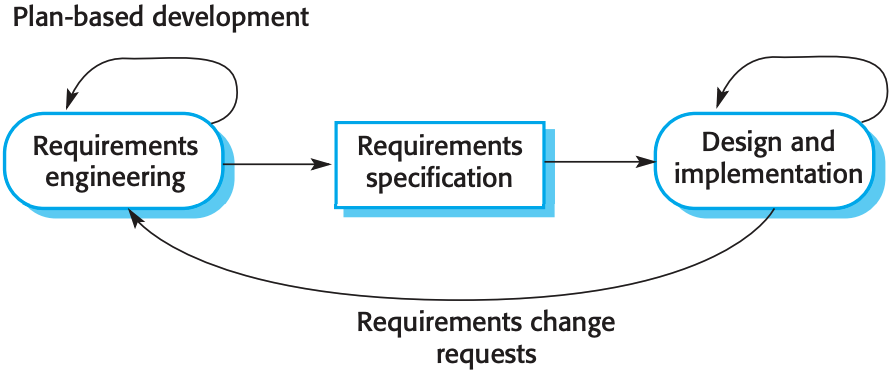
\includegraphics[width=0.6\textwidth]{6swengprocess/images/planspec.png}
    \caption{The plan-driven approach to system specification \cite{sommerville}.}
    \label{fig:planspec}
\end{figure}

As a result, the methodology chosen for development of the system was agile software development. 


\begin{figure}[H]
    \centering
    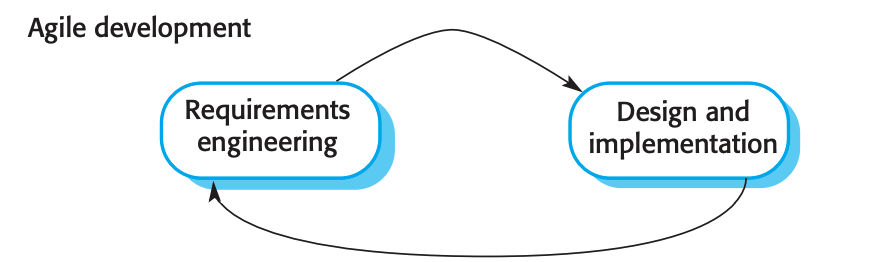
\includegraphics[width=0.6\textwidth]{6swengprocess/images/agilespec.png}
    \caption{The agile approach to system specification \cite{sommerville}.}
    \label{fig:agilespec}
\end{figure}

Agile software development is an approach which is incremental, cooperative (customer and developers working constantly together with close communication), straightforward (the method itself is easy to learn and to modify), and adaptive (able to make last moment changes) \cite{Abrahamsson}. 

The fact that increments are small and, typically, new iterations of the system are made every two or three weeks \cite{sommerville} as well as the fact that customer (supervisor) involvement is frequent throughout the process make an agile approach ideal for the project. Given the timescale, rapid feedback was critical to successful development of the codeHelper application. Figure \ref{fig:agilespec} shows the approach to system specification in agile methods and should be compared to figure \ref{fig:planspec}.

In practice, a methodology close to Scrum was followed throughout the project. 

To begin the project, there was an initial planning phase as outlined by Scrum and required by the nature of a Master's dissertation. During this phase, the architecture of the project was defined. However, during development, adjustments were made to this architecture as outlined by Scrum \cite{scrum}. During the planning phase, Trello \cite{trello} was used to store a list of currently identified tasks (see Figure \ref{fig:backlog}), known in Scrum as a backlog \cite{scrum}.

\begin{figure}[H]
    \centering
    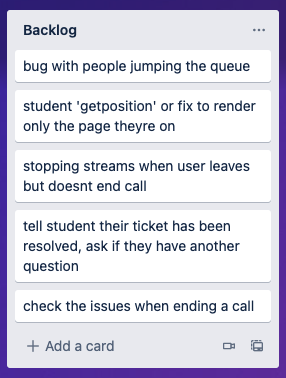
\includegraphics[width=0.4\textwidth]{6swengprocess/images/trelloBacklog.png}
    \caption{Example of scrum backlog of tasks on Trello during the project.}
    \label{fig:backlog}
\end{figure}

After minimal initial planning, Scrum purports a series of short development phases, or sprints (see Figure \ref{fig:scrum}), deliver the product incrementally \cite{scrum}. Sprints aim to produce a visible, usable product that implements one or more user interactions with the system - to deliver valuable functionality \cite{scrum}. These sprints were one week long, since the supervisor meetings were weekly. At the beginning of each sprint, tasks in the backlog were updated and prioritised before identifying the tasks that should be completed in that sprint. Tasks in the project were designed to be specific enough to be completed in a week or less (see Figure \ref{fig:backlog}). 

\begin{figure}[H]
    \centering
    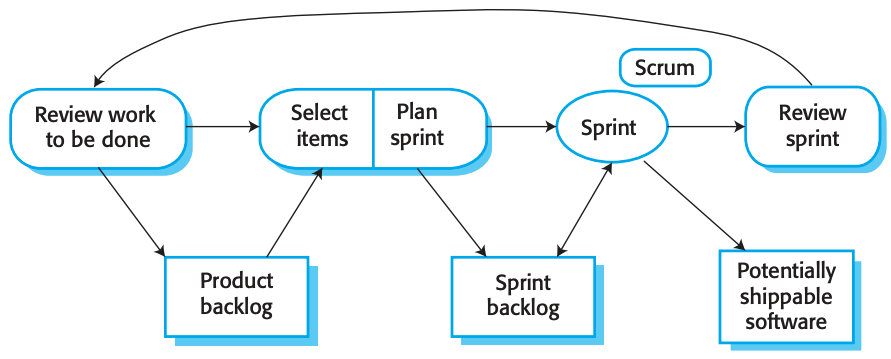
\includegraphics[width=0.65\textwidth]{6swengprocess/images/scrum.png}
    \caption{The scrum sprint cycle \cite{sommerville}.}
    \label{fig:scrum}
\end{figure}

Weekly supervisor meeting offered the chance to review each sprint, since the project supervisor is also the product owner or customer. During these meetings, project goals and tasks can be added, eliminated or reprioritised. In this project as in application of Scrum in industry, items which the customer prioritises must have the highest development priority \cite{scrum}.
\chapter{Design}
The following chapter shall discuss the planning and design choices of the system. 

\newpage
\section{TODO Sequence Diagram}

\newpage
\section{Interface}

\begin{figure}[H]
    \centering
    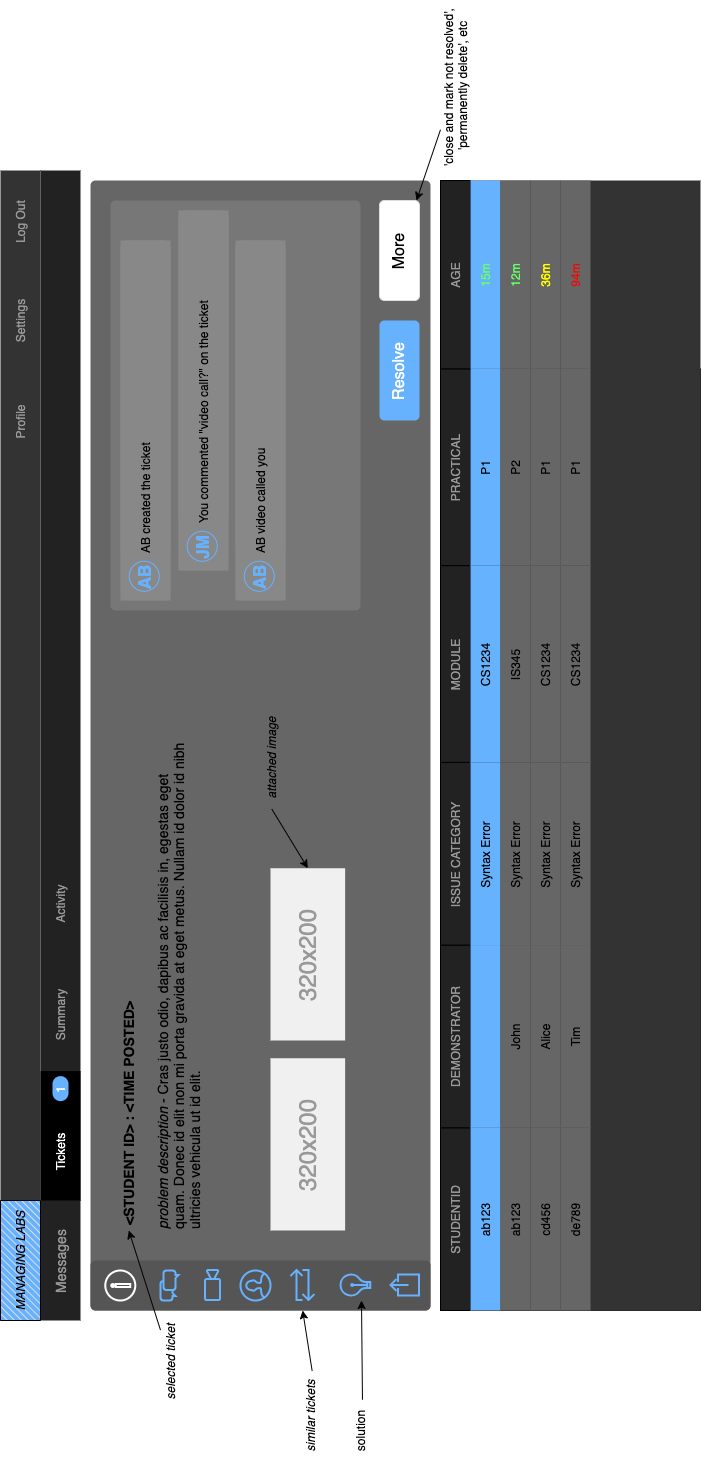
\includegraphics[width=0.6\textwidth]{7design/images/demoTickets.png}
    \caption{Simple design for the demo ticket viewing interface.}
    \label{fig:demoTickets}
\end{figure}

\section{Database}

\subsection{Entities, Attributes and Relationships}
We will now define a representation of the data in terms of entities, attributes and relationships between entities.

\subsubsection{Entities}

We represent the components of the systems as the following entities. 

\FloatBarrier
\begin{table}[H]
\centering
\begin{tabular}{ |l|c| } 
 \hline
 \textbf{Entity Set} & \textbf{Attributes}\\ 
 \hline
  user & \underline{username}, name\\ 
 \hspace{6pt}user.student & \\ 
 \hspace{6pt}user.demonstrator & \\
 \hspace{12pt}user.demonstrator.labLead & \\
 auth & \underline{username}, password, role \\
 ticket & \underline{ticketId}, issueDescription,\\
 & practical, resolutionStatus \\
 attachment & \underline{attachmentId}, file, caption \\
 lab & \underline{labId}, openTime, closeTime\\
 solution & \underline{solutionId}, solutionDescription\\
 category & \underline{name} \\
 module & \underline{moduleCode} \\
 \hline
\end{tabular}
\caption{Table of entities and associated attributes.}
\end{table}
\FloatBarrier

Primary keys are denoted as \underline{underlined}. Foreign keys are denoted in \textit{italics}.

Note that \textbf{user.student} and \textbf{user.demonstrator} are disjoint specialisations of the entity set \textbf{user} - a user is always a student or demonstrator (or specialisation of demonstrator). \textbf{user.demonstrator.labLead} is a further specialisation of \textbf{user.demonstrator}, not disjoint. 

\subsubsection{Relationships}
We shall now define the relationships between entities and the constraints on them. 

\FloatBarrier
\begin{table}[H]
\centering
\begin{tabular}{ |c|c|c|c| } 
 \hline
 \textbf{Relationship} & \textbf{Entities} & \textbf{Participation} & \textbf{Cardinality}\\ 
 \hline
 $r$ & $e_1$, $e_2$ & total, partial & M-1 \\
 \hline
\end{tabular}
\end{table}
\FloatBarrier 

We denote many as M, one as 1 such that one to many relationship would be denoted 1-M. Note that for a relationship $r$ that is many (in $e_1$) to one (in $e_2$) and has total participation from $e_1$ but partial from $e_2$ then the row in the table is written as above. Participation will be listed in order that entities are written.

\FloatBarrier
\begin{table}[htbp]
\centering
\resizebox{\columnwidth}{!}{\begin{tabular}{ |c|c|c|c|c| } 
 \hline
 \textbf{Relationship} & \textbf{Relationship Attributes} & \textbf{Entity Sets} & \textbf{Participation} & \textbf{Cardinality}\\ 
 \hline
 creates & creation\_timestamp & user.student, ticket & partial, total & 1-M \\
 assignedTo & demAssigned\_timestamp & user.demonstrator, ticket & partial, partial & 1-M\\
 writes & demSolved\_timestamp & user.demonstrator, solution & partial, total & M-M\\
 leads & & user.demonstrator.labLead, lab & partial, total & 1-M\\
 hasAttachment & ticket\_attach\_timestamp & ticket, attachment & partial, partial & 1-M\\
 hasAttachment & solution\_attach\_timestamp & solution, attachment & partial, partial & 1-M\\
 postedIn &  & ticket, lab & total, partial & M-1\\
 hasTicketCat & & ticket, category & total, partial & M-M\\
 hasSolutionCat & & solution, category & total, partial & M-M\\
 demonstratesInLab& & user.demonstrator, lab & partial, total & M-M\\
 enrolledInMod && user.student, module & total, partial & M-M\\
 demonstratesInMod && user.demonstrator, module & partial, partial & M-M\\
 leadsMod && user.ladLead, module & partial, partial & 1-M\\
 toDoWith && ticket, module & total, partial & M-1\\
 hasAuth && user, auth & total, total & 1-1 \\ 
 \hline
\end{tabular}}
\caption{Table showing entities, relationships between, relationship attributes, participation and cardinality.}
\end{table}
\FloatBarrier

\subsubsection{Entity Relationship Diagram}

\begin{figure}[H]
    \centering
    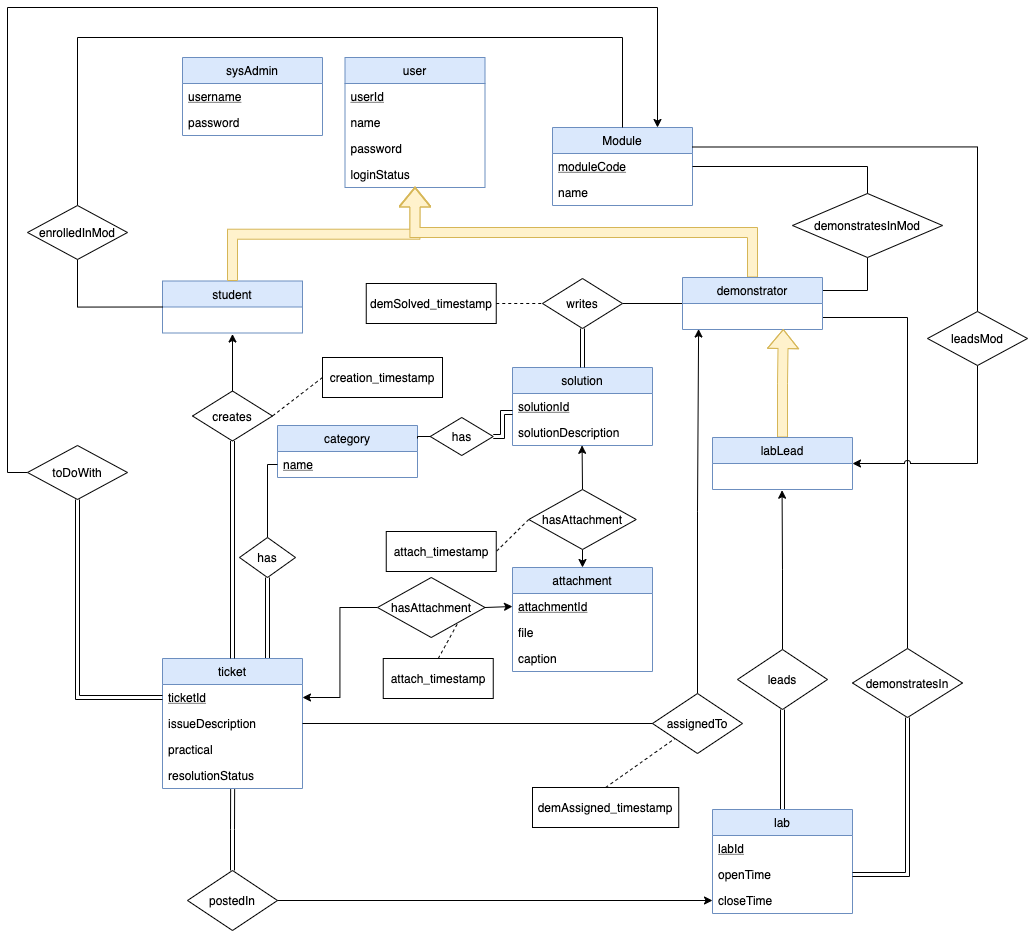
\includegraphics[width=\textwidth]{7design/images/ER.png}
    \caption{\gls{er} diagram for the system.}
    \label{fig:ER}
\end{figure}

\subsubsection{Relational Schema}
The first task is to translate the given E-R model into corresponding database schema below.\\

\noindent student - \underline{\textit{username}}, name, enrolledModules \\
demonstrator - \underline{\textit{username}}, name, demonstratedModules \\
labLead - \underline{\textit{username}}, name, demonstratedModules, ledModules \\
auth - \underline{username}, password, role \\
ticket - \underline{ticketId}, issueDescription, module, practical, resolutionStatus, \textit{student.username}, creation\_timestamp, \textit{demonstrator.username}, demAssigned\_timestamp, \textit{labId} \\
category - \underline{name} \\
solution - \underline{solutionId}, solutionDescription\\
attachment - \underline{attachmentId}, file, caption, \textit{ticketId}, ticket\_attach\_timestamp, \textit{solutionId}, solution\_attach\_timestamp\\
lab - \underline{labId}, title, openTime, closeTime, \textit{labLead.username}\\
writes - \underline{\textit{demonstrator.username}}, \underline{\textit{solutionId}}, demSolved\_timestamp\\
hasTicketCat - \underline{\textit{tickedId}}, \underline{\textit{name}}\\
hasSolutionCat - \underline{\textit{solutionId}}, \underline{\textit{name}}\\
demonstratesInLab- \underline{\textit{demonstrator.username}}, \underline{\textit{labId}}\\
module - \underline{moduleCode}, name, \textit{labLead.username}\\
enrolledInMod - \underline{\textit{student.username}}, \underline{\textit{moduleCode}}\\
demonstratesInMod - \underline{\textit{demonstrator.username}}, \underline{\textit{moduleCode}}\\

\subsubsection{Relational Schema Diagram}

\begin{figure}[H]
    \centering
    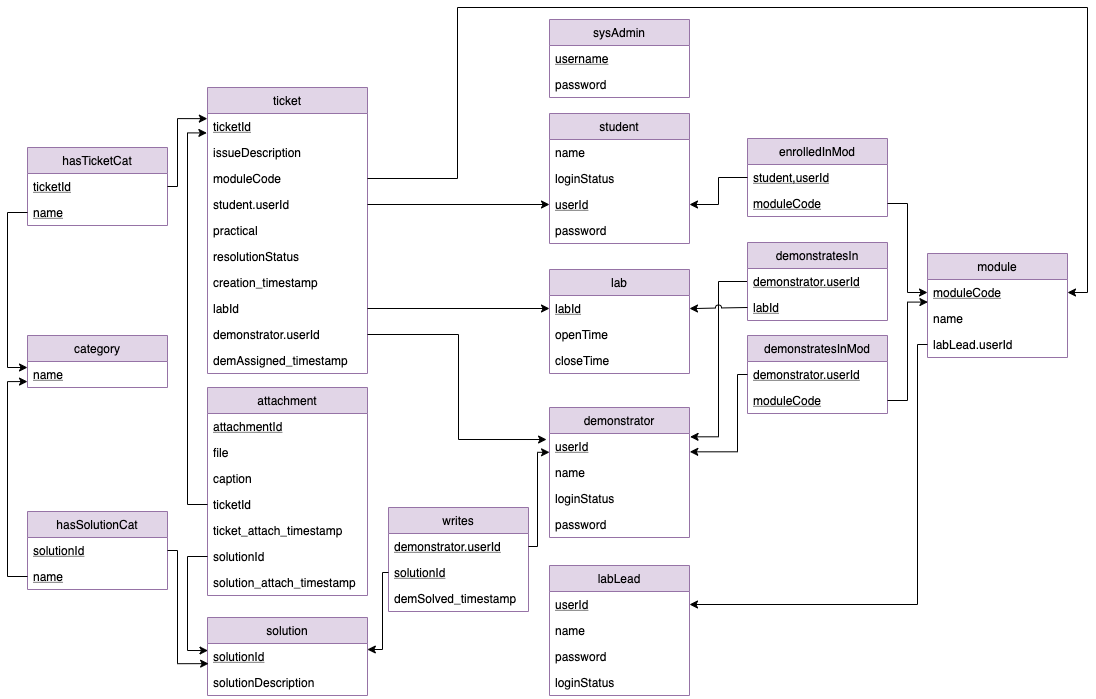
\includegraphics[width=0.8\textwidth]{7design/images/relationalSchema.png}
    \caption{Relational schema diagram for the system.}
    \label{fig:relationalschema}
\end{figure}

\subsubsection{Attribute Types}
A data type must be specified for each attribute. Table \ref{table:atypetable} below shows the attribute type for each attribute, as well as it's original, parent relational table - in other words, we do not repeat the attributes that appear as foreign keys in tables.

\begin{table}[H]
\centering
\begin{tabular}{| c | c | c | c |}
\hline
 Relational Table & Attribute & Attribute Type & Notes\\ 
 \hline
  category & name & VARCHAR(70) & Government data standards\cite{dataStandards}\\
  \hline
  ticket & ticketId & INT & Auto incremented by DB.\\
  & issueDescription & VARCHAR(2000)&\\
  & practical & VARCHAR(6)&preset list?\\
  & resolutionStatus & VARCHAR(8)&[new, missed, inProgress, closed]\\
  & creation\_timestamp & DATE &\\
  &  demAssigned\_timestamp & DATE &\\
  \hline 
  attachment & attachmentId & INT & Auto incremented by DB.\\
  & file & BLOB &\\
  & caption & VARCHAR(150) & \\
  & ticket\_attach\_timestamp & DATE &\\
  & solution\_attach\_timestamp & DATE& \\
  \hline
  solution & solutionId & INT&Auto incremented by DB.\\
  & solutionDescription & VARCHAR(2000)&\\
  \hline
  writes & demSolved\_timestamp & DATE &\\
  \hline
  sysAdmin & username & VARCHAR(16) &\\
  & password & CHAR(60) & hashed password\\
  \hline
  student & name & VARCHAR(70) & Government data standards\cite{dataStandards}\\
  & username & INT&studentnumber details?\\
  & password & CHAR(60)&hashed password\\
  \hline
  lab & labId & INT&Auto incremented by DB.\\
  & title & VARCHAR(70) & \\
  & openTime & DATE &\\
  & closeTime & DATE &\\
  \hline
  demonstrator & username & VARCHAR(16)&\\
  & name & VARCHAR(70)& Government data standards\cite{dataStandards}\\
  & password & CHAR(60) &hashed password\\
  \hline
  labLead & username & VARCHAR(16)&\\
  & name & VARCHAR(70) & Government data standards\cite{dataStandards}\\
  & password & CHAR(60)& hashed password\\
  \hline
  module & moduleCode & CHAR(6) & Fixed type [A-Z]\{2\}\arraybackslash \textbackslash d\{4\}
\\
  & name & VARCHAR(70)& Government data standards\cite{dataStandards}\\
 \hline
 
 \hline
\end{tabular}
\caption{Table describing the data types for attributes, showing the parent relational table.}
\label{table:atypetable}
\end{table}

The Government Data Standards Catalogue\cite{dataStandards} was referenced for the data types corresponding to names - including logical extension to category and module names. 

ID data types are defined as INT,auto increment from db. 

\subsection{choices}

-react / enterprise level -> load balancing
-why sql
-data access object
\chapter{Implementation}

This chapter describes the implementation of the codeHelper application. After selecting the technology stack and outlining the system architecture, user interface and workflow, the next stage of development is implementation. The implementation was carried out incrementally, as described in section \ref{sec:designreact}, based on the system requirements in Chapter \ref{chap:req}. 

\section{Client-Server Interaction}

As discussed in the Architectural Design section, section \ref{sec:architecture}, the client-side rendering model requires processing on both the client and server. As discussed in section \ref{sec:architecture}, codeHelper uses a client-server architecture. The interaction between client and server was carried out in two ways - by websockets and HTTP requests.

\subsection{Socket.io}

Socket.IO is a library that enables real-time, bidirectional and event-based communication between the browser and the server \cite{socketio}. Socket.IO is not simply a websocket implementation - it utilises websockets primarily, but can fall back to long-polling when websockets are unavailable. This is useful in our application, since it allows legacy browsers access when websockets are not supported and also an alternative if proxy, firewall or configuration issues prevent a websocket connection from being established.

HTTP long-polling transport, often called long-polling or polling, consists of successive HTTP requests \cite{socketio}. This includes both GET requests for requesting data from the server and POST requests for sending data to the server.

As well as the ability to fallback to long-polling, a key feature of Socket.io is `rooms'. A room is an arbitrary channel that sockets can join and leave that can be used to broadcast events to a subset of clients \cite{socketio}. In the codeHelper system, upon socket connection, users are assigned to rooms. All demonstrators are a member of the `demonstratorChat' room. This allows the tickets and demonstrator messages to be sent exclusively to the demonstrators. Although demonstrators are broadcast all chats in the `demonstratorChat' room (to enable them to interact in every chat via each ticket) each student's chat is broadcast from, and emitted to, the room named for that student. This allows demonstrators to communicate directly with any given student and means that students only have access to their own chat. 

Figure \ref{fig:socketiorooms} shows an example of how rooms are organised in the codeHelper application. \textit{Demonstrator1} is chatting to \textit{student1}, therefore requires access to the `student1' socket room. \textit{demonstrator2} is not chatting to any students and so does not require access to any student socket rooms. Both \textit{demonstrator1} and \textit{demonstrator2} require access to the `demonstratorChat' socket room so that they can receive tickets and demonstratorChat messages. \textit{student1} requires access to the student1 socket so as to receive their associated messages.

\begin{figure}[H]
    \centering
    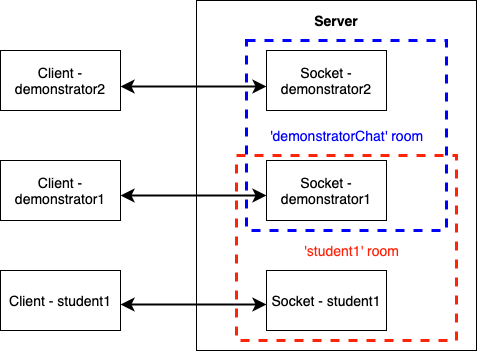
\includegraphics[width=0.6\textwidth]{8implementation/images/socketRooms.png}
    \caption{Example of the organising of Socket.io rooms in the codeHelper application.}
    \label{fig:socketiorooms}
\end{figure}

Socket.io is implemented in the areas of the application where data needs to be real-time. This includes the tickets in the demonstrator help desk, messages, student queue position, messaging and video call initiation. 

The Socket.io connection is established when the user opens the application and the connection is maintained until the application is closed. This is necessary to enable messages to be received whilst the user is at any point in the application. 

\subsection{HTTP Requests}

For data that does not require real-time updates, HTTP requests are used to send and receive data. This includes ticket solutions, summary and statistics data, user roles and student history (i.e. previous tickets).

HTTP requests are made by the client, to the host, which is located on a server. The goal of the request is to access a resource on the server. In order to create the request, the client uses components of a URL (Uniform Resource Locator), which includes the information needed to access the resource \cite{ibmhttp}. 
A HTTP request contains a request line with the request method (GET or POST), the path and the HTTP version. It also contains a series of HTTP headers with information about the message, the sender, and the form of communication. Additionally, a HTTP request can also contain a message body, which includes any input data that the user wishes to send to the server in a POST request \cite{ibmhttp}.

In the codeHelper system, HTTP requests are implemented on the client side using the Fetch API - a standard interface for fetching resources across a network \cite{fetch}. On the server side, the routing and request handling is simplified by using Express \cite{express}, as discussed in section \ref{sec:express}.

POST requests for the creation of, for example, tickets and solutions are sent when the user submits the associated form. GET requests that obtain data for populating pages, such as requesting a solution for a given ticket or requesting a list of all users for the `roles' page, are implemented using the useEffect hook in React \cite{useeffect} - posting the request when the page is accessed, updating the component state with the data and re-rendering the page to show the updated data. This allows page data to be loaded as the page is loaded, providing recent data without the need to manually request as well as reducing the network strain by downloading data only as needed.

\section{Video Calls}

Video calls and screen-sharing were implemented in-app to provide a more complete user experience, as well as to increase efficiency and minimise the surface area of error that is associated with trying to switch between multiple systems (as discussed in section \ref{sec:currentsystem}).

Video calls are implemented using \gls{webrtc}, an open-source project that supports video and voice data to be sent between peers.

The technology is available on all modern browsers and they provide regular Javascript APIs for the technologies behind it, implemented as an open web standard \cite{webrtc}. 

\subsection{PeerJS}

PeerJS is a simple wrapper for the browser's WebRTC implementation. It provides a complete and configurable peer-to-peer connection API which simplifies the browser standard. PeerJS only requires connection to a shared peer server and an ID, with which it can create a \gls{p2p} data or media stream connection to a remote peer \cite{peerjs}.

To facilitate P2P connections, PeerJS connects to a PeerServer. In the codeHelper application, the PeerServer is run on the server. No peer-to-peer data goes through the server, the server acts only as a connection broker \cite{peerjs}. Figure \ref{fig:videoactivity} shows a UML activity diagram for the process of establishing a call between a student and demonstrator using PeerJS, omitting the details of how the PeerServer creates a P2P connection.

\begin{figure}[H]
    \centering
    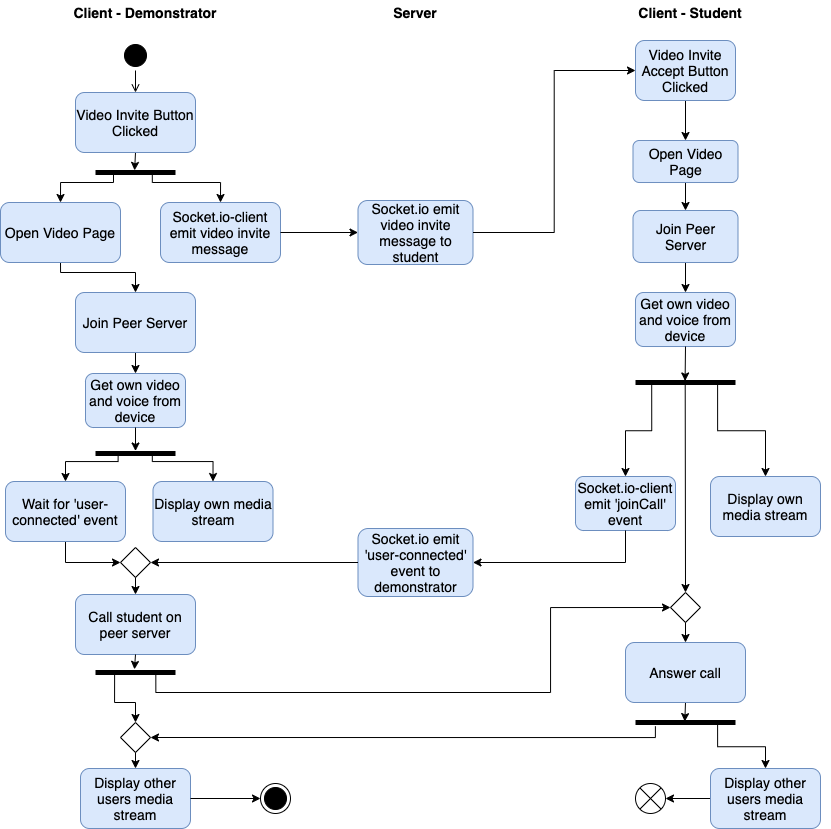
\includegraphics[width=\textwidth]{8implementation/images/activityVideoCall.png}
    \caption{UML activity diagram for a successful video call in the codeHelper application.}
    \label{fig:videoactivity}
\end{figure}

It's important to note that the P2P connection could have been used to send messages but was not. Sending messages over the P2P connection would have improved security, by minimising the risk of messages being misdirected to other users, and improved performance by reducing the traffic and processing carried out on the shared server. However, the application benefited greatly from handling messages separately on the express server since it allows demonstrators to interact with the chats on all tickets. 

\section{File Exchange}

File exchanging was implemented in order to allow students to send image, code or other files in the chat, thereby helping to provide demonstrators with more concrete information that can help them solve the issue.

Files are uploaded to the server using the already established websocket connection. This is implemented using a package called socketio-file-upload \cite{siofu}. A major design choice here was to save the files on the server, rather than to store them temporarily (as with the messages) in the chat. This was done so that demonstrators or lab leads could review files that were exchanged between students and demonstrators.

The chatKey for each chat, corresponding to the room name in Socket.io, is added to the file's meta data. Upon successful upload to the server, the server determines the \gls{mime} type of the object. If the file's MIME type indicates that it is an image, the file is converted to a base 64 string and a message object of type `image' is created and added to the chat - including the image string. This allows the image to be displayed immediately after it is sent. Otherwise, a message of type `file' will be added to the chat, which are rendered on the client side as a hyperlink. For both images and files, clicking on the hyperlink or image will post a HTTP request to the server to download the image based on its file name. Note that if multiple images are uploaded with the same name, socketio-file-upload will rename them and provide that file name to the client.

\section{Database}

The SQL database that was implemented was MariaDB, as discussed in sections \ref{sec:stackdb} and \ref{whysql}. The Node.js package used on the codeHelper server to interact with the database was MySQL2 \cite{npmmysql2}, a drop in replacement for original MySQL package which offers better performance. It was used for this project because of its new implementation of promise wrappers and pooling.

The SQL database originally selected for this project was MySQL, hence the choice of SQL client. The switch to MariaDB did not affect the choice of Node.js package since MariaDB is a drop-in, binary compatible replacement for MySQL \cite{Bartholomew} that works with MariaDB \cite{npmmariadb}.

In the final implementation, a `LoginRequests' table was created to store session information. This resulted in the schema, produced by MySQLWorkbench, show in figure \ref{fig:relationalschemafinal}.

\begin{figure}[H]
    \centering
    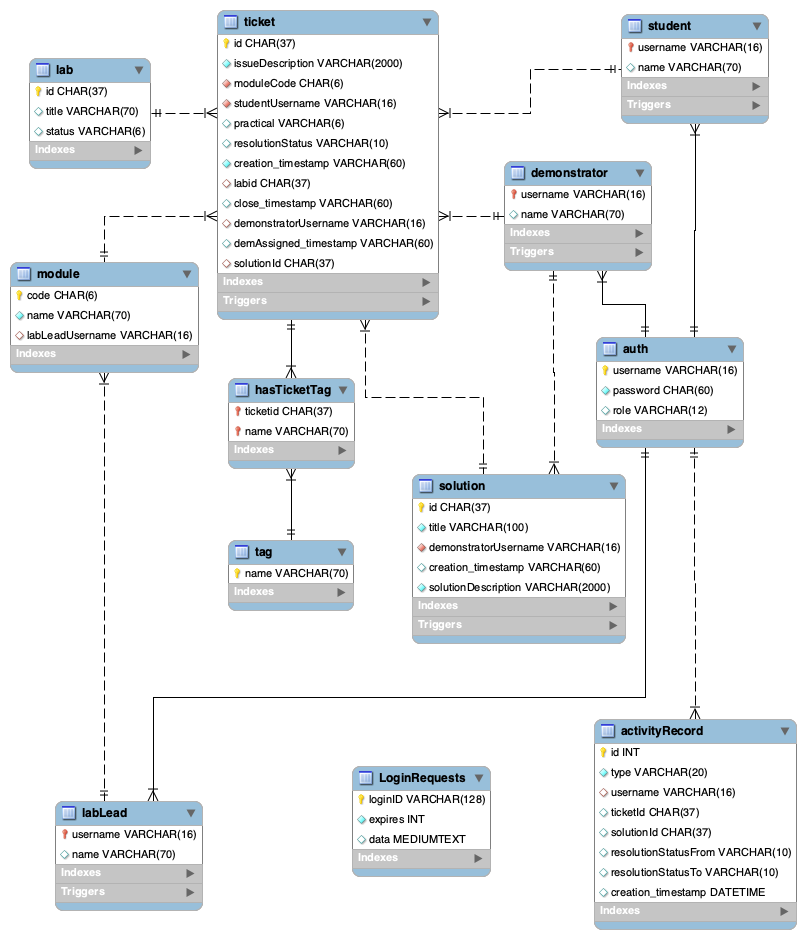
\includegraphics[width=\textwidth]{8implementation/images/schemaFinal.png}
    \caption{Final and complete schema diagram for the system.}
    \label{fig:relationalschemafinal}
\end{figure}

\subsubsection{Triggers}

A trigger is a named database object that is associated with a table, and that activates when a particular event occurs for the table. Some uses for triggers are to perform checks of values to be inserted into a table or to perform calculations on values involved in an update \cite{trigger}. 

Triggers were used for two separate tasks in the building of the codeHelper system.

\paragraph{Recording Activity}
 Triggers were used, upon adding to or editing certain tables, to add activity data to the `activityRecord' table. For example, when a row in the ticket table is updated, one of the triggers shall check if the status of the ticket is the same as it was before the update - if it is not, it shall insert a row into the `activityRecord' table with the value `ticketStatusChanged' in the type column.

\paragraph{Ensuring Demonstrator Privileges} - A trigger is also used to ensure that lab lead accounts also have the privileges of demonstrators. To ensure data consistency, some tables reference the username of users in the demonstrator table. The use of the trigger here allows lab leads to not only perform system administration and view statistics, but also allows them to be able to act as demonstrators in assigning themselves to tickets.

\subsubsection{Attribute Types}
A data type must be specified for each attribute. Table \ref{table:atypetable} below shows the attribute type for each attribute, as well as it's original, parent relational table - in other words, attributes that appear as foreign keys in tables are not repeated.

\begin{table}[H]
\centering
\resizebox{\columnwidth}{!}{%
\begin{tabular}{| c | c | c | c |}
\hline
 Relational Table & Attribute & Attribute Type & Notes\\ 
 \hline
  tag & name & VARCHAR(70) & Government data standards\cite{dataStandards}\\
  \hline
  ticket & ticketId & CHAR(37) & Unique identifier \cite{uuid} prefixed with `T'.\\
  & issueDescription & VARCHAR(2000)&\\
  & practical & VARCHAR(30)& \\
  & resolutionStatus & VARCHAR(10)&[new, missed, inProgress, closed]\\
  & creation\_timestamp & DATE &\\
  &  demAssigned\_timestamp & DATE &\\
  \hline
  solution & solutionId & INT &  Unique identifier \cite{uuid} prefixed with `S'.\\
  & solutionDescription & VARCHAR(2000)&\\
  \hline
  auth & username & VARCHAR(16) & \\
  & password & CHAR(60) & Hashed password. \\
  & role & VARCHAR(12) & [student, demonstrator, labLead] \\
  \hline
  lab & labId & INT& Unique identifier \cite{uuid} prefixed with `L'.\\
  & title & VARCHAR(70) & \\
& status & VARCHAR(6) & [open, closed] \\
  \hline
  user & name & VARCHAR(70)& Government data standards\cite{dataStandards}\\
  \hline
  module & moduleCode & CHAR(6) & Fixed type [A-Z]\{2\}\arraybackslash \textbackslash d\{4\}
\\
  & name & VARCHAR(70)& Government data standards\cite{dataStandards}\\
 \hline
 
 \hline
\end{tabular}}
\caption{Table describing the data types for attributes, showing the parent relational table.}
\label{table:atypetable}
\end{table}

The Government Data Standards Catalogue\cite{dataStandards} was referenced for the data types corresponding to names - including logical extension to category and module names. 

\subsubsection{Data Access Object}

The \gls{dao} pattern was used to create a separation between data access logic and the main application logic. This makes it significantly easier to replace or modify an application's data resources \cite{daooracle} that may arise in future refactoring or adaptation. 

There are three key benefits to implementing the use of a DAO \cite{daooracle}:

\begin{itemize}
    \item Separation of the data resource's client interface from its data access mechanisms
    \item Adapation of a specific data resource's access API to a generic client interface
    \item Allowing data access mechanisms to change independently of the rest of the system
\end{itemize}

\section{Authentication}

Authentication in the application is implemented using PassportJS, an authentication middleware for Node which authenticates requests. 

\subsection{PassportJS}

In Passport, a `local' strategy was used, meaning Passport verifies user credentials against a store of users in the database. Implementation of Passport allows the system to be adapted for the use of different strategies - including single sign-on using an OAuth provider such as Facebook or Twitter, both of which have become popular authentication methods \cite{passport}. 

\subsubsection{HTTP Requests}

\begin{figure}[H]
    \centering
    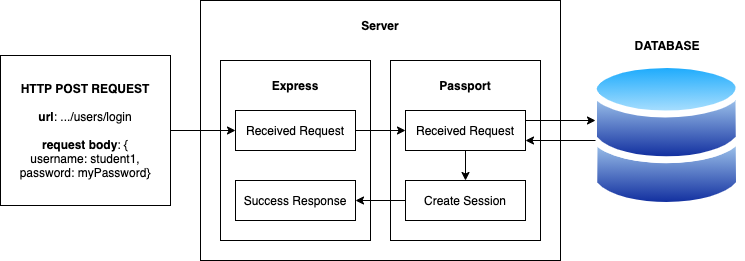
\includegraphics[width=\textwidth]{8implementation/images/passport.png}
    \caption{Basic flow of data for login using Passport.}
    \label{fig:passportlogin}
\end{figure}

Figure \ref{fig:passportlogin} shows an extremely simplified version of the basic flow of data for a user who logs in using Passport. The following steps are carried out when a user attempts to login:
\begin{enumerate}
    \item The user submits the login form, sending a HTTP POST request to .../users/login with the username and password contained in the request body.
    \item The passport.authenticate middleware is called, verifying the user by checking the user's posted credentials against the encrypted credentials stored in the database.
    \item Passport.authenticate passes the user (with hashed password) object, along with any errors or additional info (if added).
    \item If the authentication was passed, Passport will automatically log the user in by calling req.login - a functino that passport has attached to the object express uses to represent the HTTP request.
    \item Passport will use the custom serialize function to attach data to request object, in our case only the user's username.
    \item Express sends a response with status 200 the username, role and message - or, if not authenticated, a 401 response with an invalid credentials message.
\end{enumerate}

For any further requests:

\begin{enumerate}
    \item Express accesses the session data in the database and attaches it to the request. Passport is able to access the serialised user object in the request.
    \item Passport.session is invoked, checking for a serialised user object in the session.
    \item Passport.session calls the custom deserialise function, finding the user and passing them to the next middleware - it acts as a middleware which takes the request object and converts the session id (from the client cookie) into the true deserialized user object that was specified.
    \item A custom middleware function checks that the user has the required role to access the API endpoint by checking the deserialized user object.
\end{enumerate} 

\subsubsection{Socket.io}

The Websockets also implement Passport JS as a middleware, in the same way as HTTP requests do shown in figure \ref{fig:passportlogin}. 

Further, misuse by students in Socket.io is prevented by not reading the `chat' argument sent by students - whereas demonstrators specify the chat so as to be able to participate in multiple conversations. For example, when a chat message is sent to the server it has the properties `text' (containing the message text) and `chat' (specifying which chat the message is sent to) - however the chat property is only read if the user is not a student. See figure \ref{fig:socketchat}.

\begin{figure}[H]
    \centering
    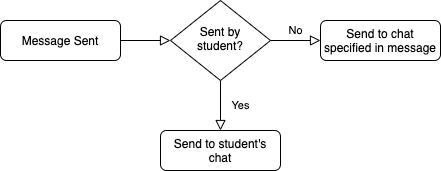
\includegraphics[width=0.7\textwidth]{8implementation/images/socketiochat.png}
    \caption{Flowchart describing logic for processing incoming chats.}
    \label{fig:socketchat}
\end{figure}

This works because students have access to, and are associated with, only their own chat, whereas demonstrators can interact with any student chat.

Additionally, Passport JS is used to authenticate socket connection requests and to assign socket usernames. The basic process is shown in figure \ref{fig:socketpassport}. By authenticating Socket.io connections with passport, the authentication of the codeHelper application is consistent. The original implementation followed the same process for setting a username as online documentation \cite{socketpassport}, by attaching the username as meta data on the socket request. The revised method of setting usernames on the server side is more secure, as it prevents users from `listening' to data on others' socket connections - which could include all of the application's tickets and messages.

\begin{figure}[H]
    \centering
    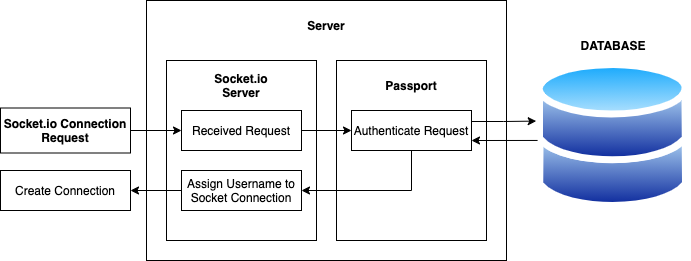
\includegraphics[width=\textwidth]{8implementation/images/socketPassport.png}
    \caption{Process of authenticating websocket connection and assigning username.}
    \label{fig:socketpassport}
\end{figure}
\chapter{Conclusion}
\chapter{Evaluation}
An evaluation experiment was carried out to test and evaluate the project. This was carried out in order to collect data about the usability of the system for those with no experience of it. 

\section{User Evaluation}\label{sec:experiment}

\subsection{Ethical Considerations}

For the evaluation to be carried out, a full ethical application was submitted to the ethics committee. 

The goal for the evaluation was to collect feedback on the custom-built online system that allows students to receive help on practical programming assignments. Participants had to be computing or IT students at the University of St Andrews and were to be recruited via emails sent to School mailing lists. Some participants were to act as ‘students’, posting representative questions about programming assignments, while others were to act as ‘demonstrators’ providing answers to questions. Participants acting as students were able to take part in text-based or video/audio chats with those acting as teachers. No chat text or video/audio data was to be stored after the chat was over. After using the system, participants were asked to complete a survey (hosted on Qualtrics) about the system. Data was be anonymous at the point of collection. Anonymous data was stored on the Qualtrics server and my University OneDrive space.
The system was hosted on the School server, ensuring that the risk of potential harms is mitigated in line with the standard School security measures.

The main ethical considerations were confidentiality, sharing personal data, and inappropriate/offensive communication between participants. Risks were mitigated by informing participants that: their participation may be known by other members of the study they communicate with via text or video/audio; participation in video/audio calls is optional; they should not share any personal information in communications; they must adhere to the code of conduct that was supplied in all communications; and they can leave the study at any time without detriment.
Participants were given pre-generated login information, meaning that any stored data, such as survey responses, content posted in the system and timing information was not able to be linked back to an identifiable individual. The system does not and did not store or process video/audio data beyond what is needed to facilitate video/audio calls.

The full ethics application was submitted and approved (approval code: CS15663). The ethical application letter is attached in appendix \ref{chap:ethicapp}.

\subsection{Participants}

Volunteers were obtained by emailing the School of Computer Science mailing list and recruiting respondents. This method of recruiting participants was particularly appropriate as it recruited students of the School - those who have an interest in a system such as codeHelper as it could help to improve their learning experience. As well as students, some of the study volunteers were those with experience as class demonstrators in the current system. This was particularly useful since they were able to analyse the codeHelper system in comparison with the current system, doing so with experience and awareness of past problems and the functionality that they would like. 

Four student volunteers and four demonstrator volunteers were obtained. Each demonstrator volunteer simultaneously volunteered as a student. This allowed demonstrators to consider codeHelper's efficacy from both `sides', and meant that there were effectively 12 active users in the user study and 12 survey participants. Although the number of participants is low, it allows initial conclusions to be drawn and points to areas that need investigation in a larger study.

\subsection{Procedure}

The evaluation experiment was 30 minutes long. It involved a 20 minute test of the system and then 10 minutes was allocated to the participants to fill out a questionnaire.

Participants were required to access the system from a web address hosted on the School server before logging into the system with login details provided. Participants from the student body were then asked to post tickets asking for help - they were provided with 2 sample problem scenarios, including code files and issue screenshots. Participants from the class demonstrator body were asked to follow the process of resolving these tickets, with an emphasis on trying out various aspects of the system such as the video and screen sharing features (if the student was willing), solution editing, assigning and creation as well as viewing the summary and statistics data page. Participants from the class demonstrator body were also provided with information required for them to participate as students in a second browser window if they wished, giving them the opportunity to test the system from the student side given that their experience and opinion was so valuable.

No specification about which browser to use was made, given that attention was paid to making the application compatible with various modern and legacy browsers. This was important, as it would not be possible to specify students use a specific browser if the system were to make it to production.

A deliberate choice was made not to provide instructions or training for the system. The codeHelper system was designed to be intuitive, simple and easy to use and so by not providing instructions it allowed part of the evaluation to gain insight into whether these goals had been achieved.

\subsection{Results}

Responses were collected from the eight participants in the experiment. The results from these questionnaires are presented in the following section.

\subsubsection{Students}

Students found the system easy to use, with all respondents finding it extremely easy to post a question, use text chat, and use screen sharing, and all respondents finding it extremely or somewhat easy to use the file sharing feature. The video chat had more mixed results, with 2 thirds finding it easy to use, and 1 third finding it somewhat difficult. All respondents found the workflow extremely or somewhat natural, found the system extremely or somewhat easy to use overall and liked the overall look and feel somewhat or a great deal. 

Respondents' comments were mostly minor feature or styling suggestions, suggesting that the overall system functionality and workflow was not an issue.

For the 8 participants acting as students, the questionnaire responses are given below. 

\begin{figure}[H]
    \centering
    \textbf{1. How easy did you find it to post a question?}\par\medskip
    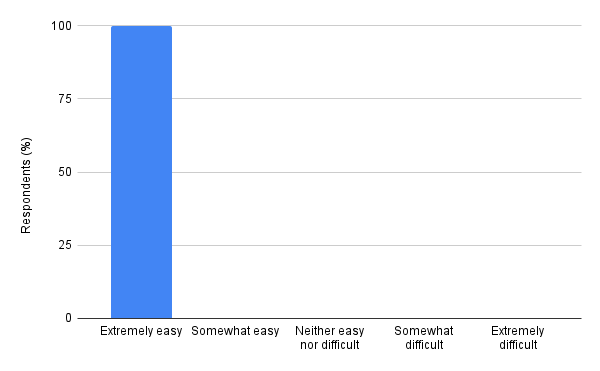
\includegraphics[width=0.75\textwidth]{10evaluation/images/stud1.png}
    \caption{Student participants responses concerning ease of posting a question.}
    \label{fig:stud1}
\end{figure}

\begin{figure}[H]
    \centering
    \textbf{2. Did you feel that you were aware of the demonstrators active presence on the system?}\par\medskip
    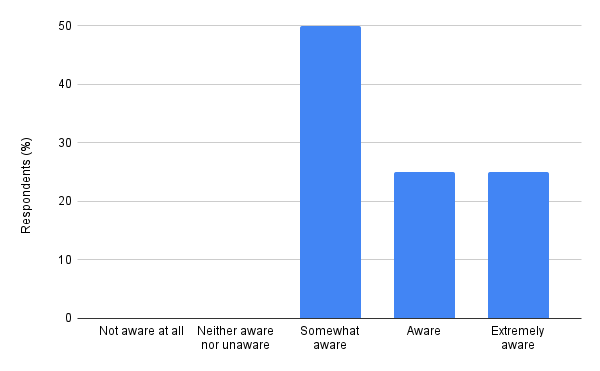
\includegraphics[width=0.75\textwidth]{10evaluation/images/stud2.png}
    \caption{Student participants responses concerning perceived awareness of demonstrators.}
    \label{fig:stud2}
\end{figure}

\begin{figure}[H]
    \centering
    \textbf{3. How satisfied were you with the `x people ahead of you in the queue' as a means of conveying wait time?}\par\medskip
    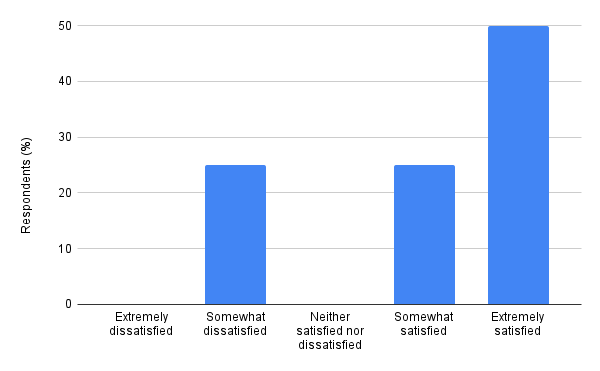
\includegraphics[width=0.75\textwidth]{10evaluation/images/stud3.png}
    \caption{Student participants responses concerning satisfaction with queue method.}
    \label{fig:stud3}
\end{figure}

\begin{figure}[H]
    \centering
    \textbf{4. How natural does the workflow, from posting a ticket to having the ticket marked as resolved, feel?}\par\medskip
    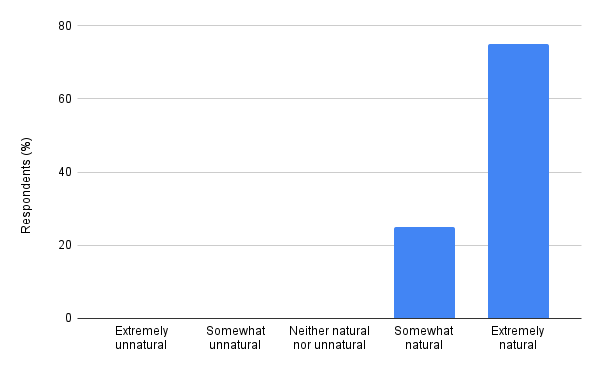
\includegraphics[width=0.75\textwidth]{10evaluation/images/stud4.png}
    \caption{Student participants responses concerning perceived naturalness of workflow.}
    \label{fig:stud4}
\end{figure}

\begin{figure}[H]
    \centering
    \textbf{5. How easy did you find using the video chat communications aspect of the system?}\par\medskip
    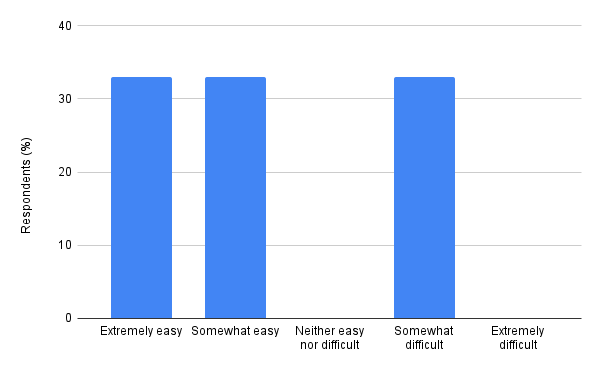
\includegraphics[width=0.75\textwidth]{10evaluation/images/stud5.png}
    \caption{Student participants responses concerning perceived ease of using video communication.}
    \label{fig:stud5}
\end{figure}

\begin{figure}[H]
    \centering
    \textbf{6. How easy did you find using the text chat communications aspect of the system?}\par\medskip
    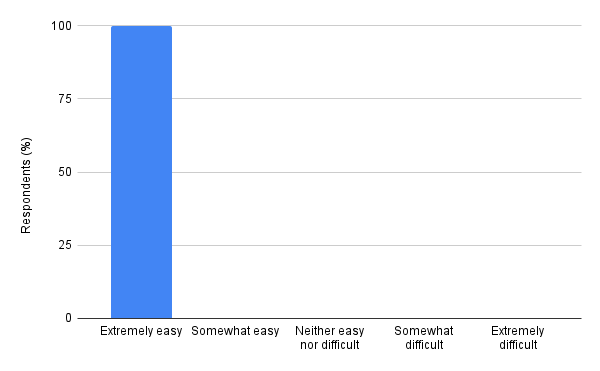
\includegraphics[width=0.75\textwidth]{10evaluation/images/stud6.png}
    \caption{Student participants responses concerning perceived ease of text chat communication.}
    \label{fig:stud6}
\end{figure}

\begin{figure}[H]
    \centering
    \textbf{7. How easy did you find using the file sharing communications aspect of the system?}\par\medskip
    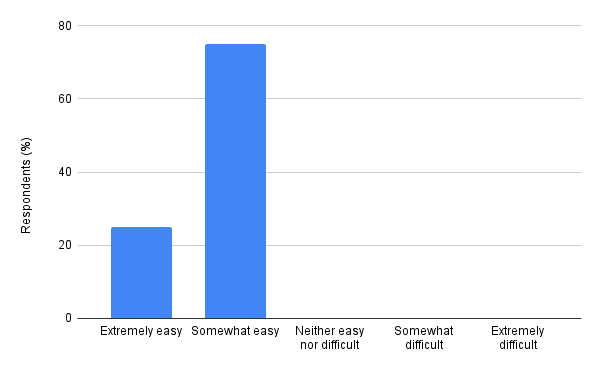
\includegraphics[width=0.75\textwidth]{10evaluation/images/stud7.png}
    \caption{Student participants responses concerning perceived ease of file sharing communication.}
    \label{fig:stud7}
\end{figure}

\begin{figure}[H]
    \centering
    \textbf{8. How easy did you find using the screensharing communications aspect of the system?}\par\medskip
    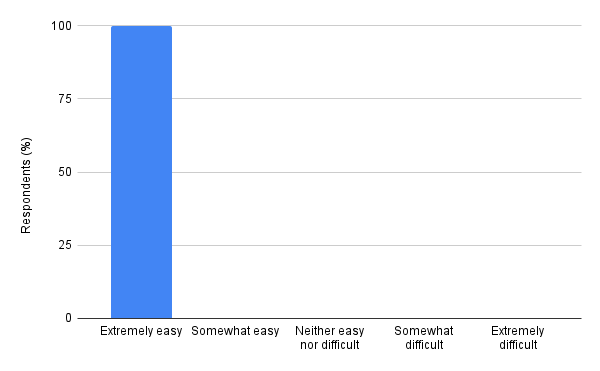
\includegraphics[width=0.75\textwidth]{10evaluation/images/stud8.png}
    \caption{Student participants responses concerning perceived ease screensharing sharing communication.}
    \label{fig:stud8}
\end{figure}

\textbf{9. Do you have any further notes or feedback on the communication aspect of system?}\par\medskip

The most notable pieces of non-positive feedback for this question were:

\begin{itemize}
    \item Consider breaking down the ticket posting form description field into "What's the problem", "What you've tried" and "Code".
    \item It might be useful to have the queue also display something like "there are currently N active sessions".
    \item For the file sharing, Ctrl+V or drag\&drop would be nice.
    \item It might be helpful to have hover over descriptions for the buttons, I was not sure what the arrow button under the call window did.
\end{itemize}

There was also a report of a `false start' with the video for one respondent. This issue has been addressed since the evaluation. Following the evaluation, all of the icon buttons had tooltips added to describe their function.

\textbf{10. Do you have any additional comments or suggestions on the ticket resolution workflow?}\par\medskip

The most notable pieces of non-positive feedback for this question were:

\begin{itemize}
    \item When waiting in the queue it would be nice to see how many lab leads are online in addition to the number of tickets in the queue.
    \item The ticket I posted was resolved, but I was surprised that I did not receive a success message, but got redirected to the starting page straight away.
    \item Have the "close ticket" box display that text in addition to the cross. I thought it would just close the session/window, and not the ticket itself. Possibly also color it green or red?	
\end{itemize}

Following the evaluation, the success message page was implemented as well as changing the `close ticket' icon box/button to a tick rather than a cross and a descriptive tooltip and colouring were added. 

\begin{figure}[H]
    \centering
    \textbf{11. How do you feel about the overall look and feel of the system?}\par\medskip
    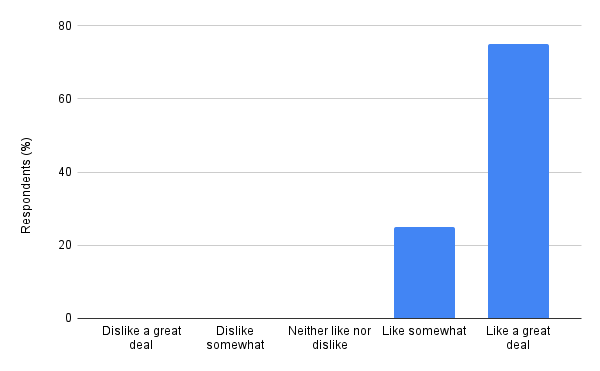
\includegraphics[width=0.75\textwidth]{10evaluation/images/stud11.png}
    \caption{Student participants responses concerning perceived look and feel of the system.}
    \label{fig:stud11}
\end{figure}

\begin{figure}[H]
    \centering
    \textbf{12. Overall, how easy would you say the system is to use?}\par\medskip
    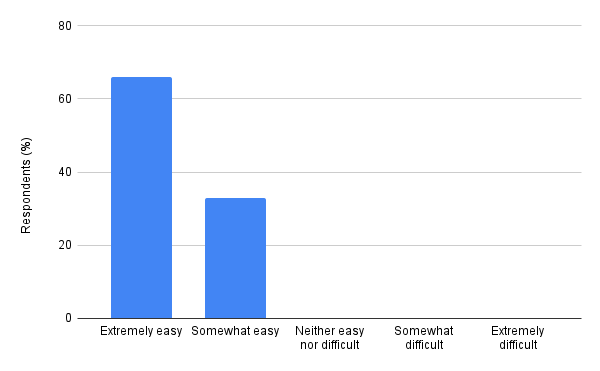
\includegraphics[width=0.75\textwidth]{10evaluation/images/stud12.png}
    \caption{Student participants responses concerning perceived overall ease of using the system.}
    \label{fig:stud12}
\end{figure}

\textbf{13. Do you have any further notes or feedback on the system?}\par\medskip

The most notable pieces of non-positive feedback for this question were:

\begin{itemize}
    \item One small remark: I was irritated by the input limit on the subject input field. I was trying to write a small description, something like "P1 - sayHello method of object syntax error", but only then figured that I was meant to write "P1" only.
    \item The chat window resizes awkwardly when starting a video call if the browser window is half-size of the screen. Might be worth resizing to the bottom in these cases.	
    \item The text input is limited for how my problem is called (Pract2), character limit at 6 was a bit confusing to describe my problem.
    \item For the problem description I would have liked some more guidance on what to type, such as "expected behaviour", "actual behaviour", or some questions that need to be answered, e.g. coding environment (might help? idk) in a field.
\end{itemize}

Following the evaluation, the limit on the `Practical' input field was increased. The chat window resizing was a key point, and should be noted for further work.

\subsubsection{Demonstrators}

Demonstrators also found the system easy to use, with all respondents finding it extremely easy to identify new tickets, assign themselves to tickets, initiate communication with the student, initiate a text chat and found it extremely or somewhat easy to initiate video calls and manage multiple tickets at once. The solution providing aspect of the system had more mixed results, with half of the participants finding it extremely easy but the other half finding it neither easy nor difficult. Demonstrators appreciated the overall system, with all respondents finding the workflow extremely natural, codeHelper `much better' than the current system, extremely easy to use overall and said they were somewhat satisfied with the overall look and feel.

For the 4 participants acting as demonstrators, the questionnaire responses are given below. 

\begin{figure}[H]
    \centering
    \textbf{1. How easy did you find it to identify a new, open ticket?}\par\medskip
    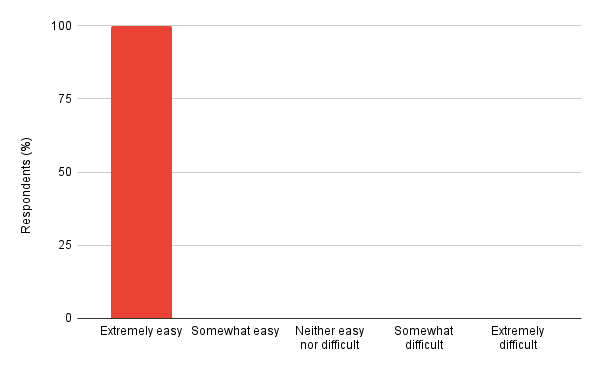
\includegraphics[width=0.75\textwidth]{10evaluation/images/dem1.png}
    \caption{Demonstrator participants responses concerning perceived ease of identifying new, live tickets.}
    \label{fig:dem1}
\end{figure}

\begin{figure}[H]
    \centering
    \textbf{2. How easy did you find it to assign a ticket to yourself?}\par\medskip
    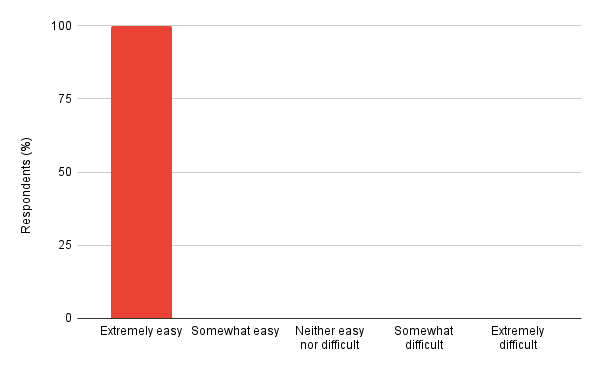
\includegraphics[width=0.75\textwidth]{10evaluation/images/dem2.png}
    \caption{Demonstrator participants responses concerning perceived ease of assigning themselves to a ticket.}
    \label{fig:dem2}
\end{figure}

\begin{figure}[H]
    \centering
    \textbf{3. How easy did you find it to initiate communication with the student?}\par\medskip
    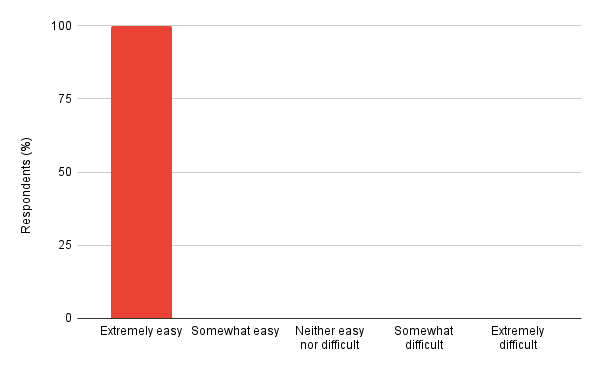
\includegraphics[width=0.75\textwidth]{10evaluation/images/dem3.png}
    \caption{Demonstrator participants responses concerning perceived ease of initiating communication with a student.}
    \label{fig:dem3}
\end{figure}

\begin{figure}[H]
    \centering
    \textbf{4. How easy did you find it to initiate a text chat?}\par\medskip
    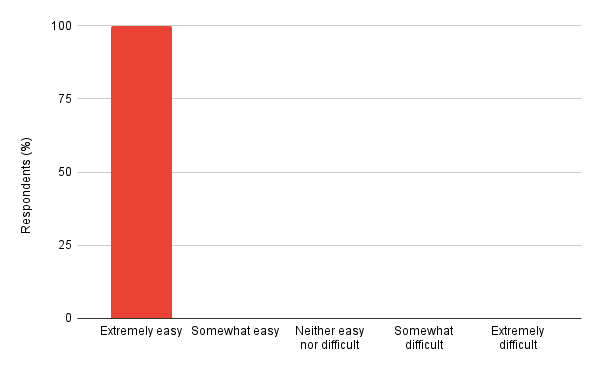
\includegraphics[width=0.75\textwidth]{10evaluation/images/dem4.png}
    \caption{Demonstrator participants responses concerning perceived ease of initiating a text chat.}
    \label{fig:dem4}
\end{figure}

\begin{figure}[H]
    \centering
    \textbf{5. How easy did you find it to initiate a video chat?}\par\medskip
    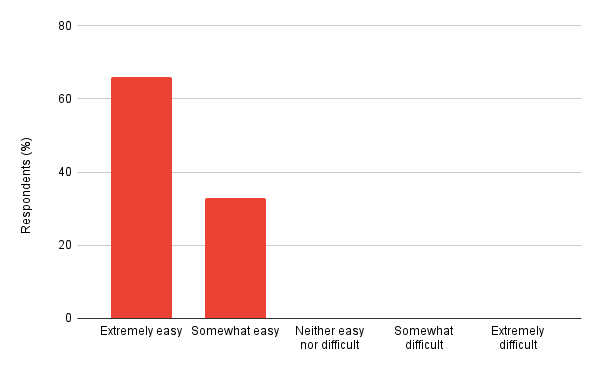
\includegraphics[width=0.75\textwidth]{10evaluation/images/dem5.png}
    \caption{Demonstrator participants responses concerning perceived ease of initiating video communication.}
    \label{fig:dem5}
\end{figure}

\begin{figure}[H]
    \centering
    \textbf{6. How easy did you find it to manage multiples tickets and chats at the same time?}\par\medskip
    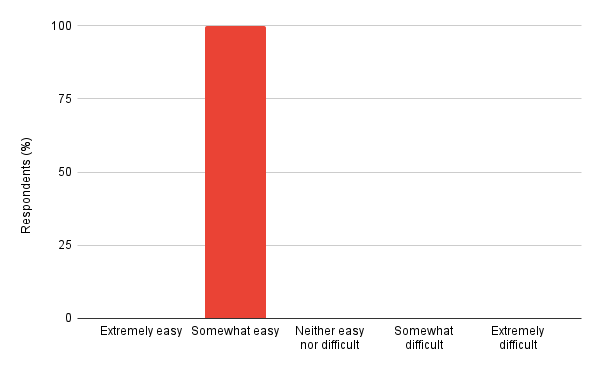
\includegraphics[width=0.75\textwidth]{10evaluation/images/dem6.png}
    \caption{Demonstrator participants responses concerning perceived ease of managing multiple tickets at once.}
    \label{fig:dem6}
\end{figure}

\begin{figure}[H]
    \centering
    \textbf{8. How easy did you find the solution providing aspect of the system?}\par\medskip
    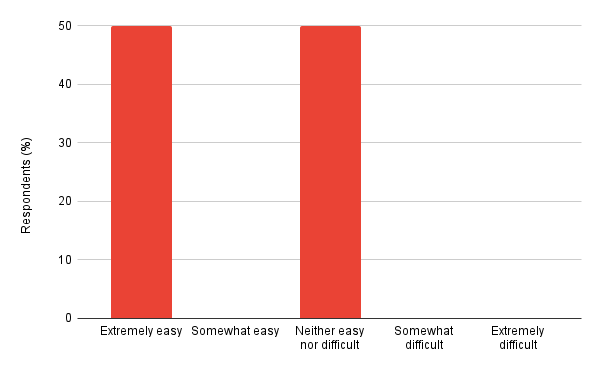
\includegraphics[width=0.75\textwidth]{10evaluation/images/dem8.png}
    \caption{Demonstrator participants responses concerning perceived ease of using the solution providing aspect of the system.}
    \label{fig:dem8}
\end{figure}

\textbf{10. Do you have any further notes or feedback on the communication aspect of system?}\par\medskip

The most notable pieces of non-positive feedback for this question were:

\begin{itemize}
    \item Have the "close ticket" button display that text along with the 'X'. I thought it would close the current window/chat rather than the whole ticket. Maybe also colour it green or red?	
\end{itemize}

\begin{figure}[H]
    \centering
    \textbf{16. How natural does the workflow, from a new ticket being posted to marking the ticket as resolved and posting a solution, feel?}\par\medskip
    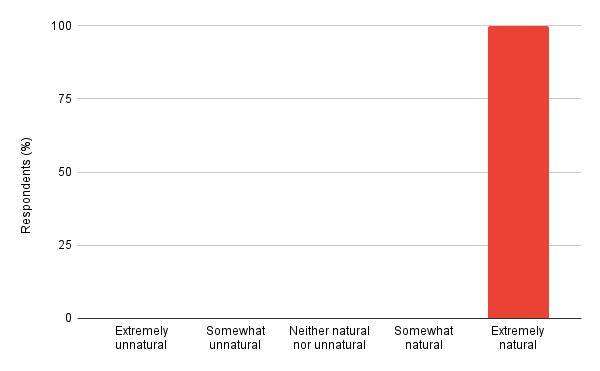
\includegraphics[width=0.75\textwidth]{10evaluation/images/dem(2)1.png}
    \caption{Demonstrator participants responses concerning perceived naturalness of workflow.}
    \label{fig:dem16}
\end{figure}

\begin{figure}[H]
    \centering
    \textbf{18. How does the system compare to the current form/list/teams based solution?}\par\medskip
    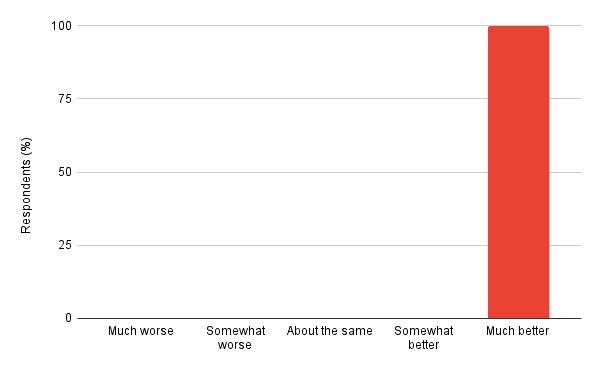
\includegraphics[width=0.75\textwidth]{10evaluation/images/dem(2)3.png}
    \caption{Demonstrator participants responses concerning perceived relative comparison with current system.}
    \label{fig:dem18}
\end{figure}

\begin{figure}[H]
    \centering
    \textbf{19. How do you feel about the overall look and feel of the system?}\par\medskip
    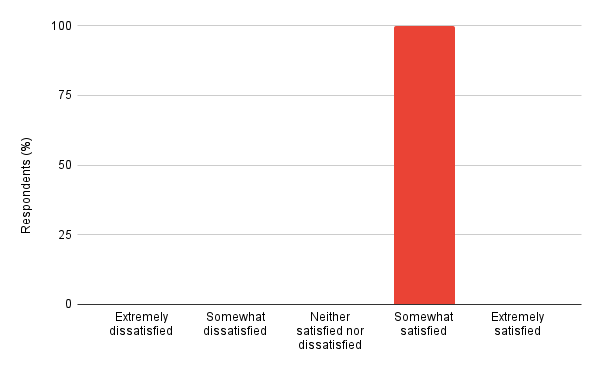
\includegraphics[width=0.75\textwidth]{10evaluation/images/dem(2)4.png}
    \caption{Demonstrator participants responses concerning perceived look and feel of the system.}
    \label{fig:dem19}
\end{figure}

\begin{figure}[H]
    \centering
    \textbf{29. Overall, how easy would you say the system is to use?}\par\medskip
    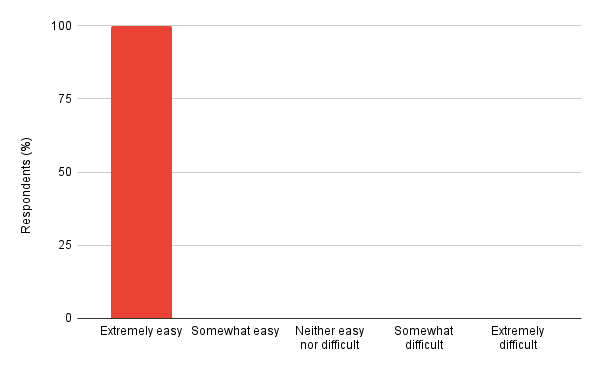
\includegraphics[width=0.75\textwidth]{10evaluation/images/dem(2)5.png}
    \caption{Demonstrator participants responses concerning perceived overall ease of using the system.}
    \label{fig:dem29}
\end{figure}

\subsection{Discussion} \label{sec:discusseval}

In this section, the results of the experiment are discussed and used to evaluate the design choices against Lauesen's usability factors \cite{lauesen} that were outlined as the design objectives of the application (discussed in section \ref{sec:interface}).

\subsubsection{Lauesen's Usability Factors}

    \paragraph{Fit for Use} From the student's perspective, the system appears to support the tasks that the user has in real life. 100\% of respondents found posting a question, using screensharing and using livechat `extremely easy', 75\% found the workflow extremely natural and 25\% found it somewhat natural, the majority of users found the video chat at least somewhat easy (and the response that it was `somewhat difficult' is likely related to the bug that was reported and fixed) and 100\% of respondents found file sharing at least `somewhat easy'.
    From the demonstrator's perspective, the system (again) appears to support the tasks. 100\% of respondents found it easy to identify new tickets, assign themselves to tickets, initiate communication, initiate a text chat specifically and also to use the system overall. 100\% of respondents found it at least somewhat easy to initiate a video chat and 100\% of respondents found managing multiple tickets/chats simultaneously somewhat easy. 
    The actions discussed above are all of the key components required by participants to communicate with others and work to resolve issues, the task that the system is to support.
    
    \paragraph{Ease of Learning, Remembering and Understandability} 100\% of demonstrators and 66\% of students found the overall system extremely easy to use, with the remaining 33\% of students finding it somewhat easy. This response is after a first use of the system in a 20 minute test, with no training or instruction of how to use the system.
    
    \paragraph{Task Efficiency} For students, 75\% of respondents found the workflow extremely natural, with the remaining 25\% finding it somewhat natural. 
    For demonstrators, 100\% found the workflow extremely natural and found managing multiple tickets/chats somewhat easy. 
    These responses, alongside previously discussed ease and satisfaction responses to communication, would appear to suggest that participants found the process to be efficient. One thing to note is that 50\% of respondents found the solution aspect of the system neither easy nor difficult - if this aspect of the system were to be improved then it would increase efficiency by increasing demonstrators use of the reusable solutions.
    
    \paragraph{Subjective Satisfaction} 100\% of demonstrator respondents were somewhat satisfied with the overall look and feel of the system, 75\% of student respondents were extremely satisfied and 25\% were somewhat satisfied. 
    These responses suggest that users were satisfied with the overall system. Although there is room for improvement on this front, it is likely related to the fact that the system was built under time constraints and is more a proof-of-concept than production build - future work on `tidying' some of the features as well as greater experience using the system in practice would reveal opportunities to improve user satisfaction.

\subsubsection{Notes}

Note that some questions were omitted from the evaluation discussion as they did not receive any responses.

Questions regarding the summary and statistics section did not receive any responses. This is likely because, although given lab lead privileges in order to view the section, the volunteers were acting as demonstrators and had knowledge and experience in this area. As a result, they did not seek out the statistics section because they would not in real life. Additionally, the statistics section only contained the small amount of data collected in the experiment and therefore did not provide much insight.

Questions regarding `non-responsive students' were also not answered. This is likely resulting from the fact that no demonstrator had experience with non-responsive students during the experiment.

\newpage
\section{Customer Feedback} 

The customer, dissertation supervisor, provided the following feedback:

``\textit{System does exactly what I was hoping for. I am very pleased the video/screenshare functionality was integrated into the webapp. Overall, it provides a much slicker and neater way of managing labs. The statistics are a great addition. The one change/addition I would like, is to be able to select which graphs to display and to be able to export the graphs/data. Also, I would have liked a prompt before closing a ticket to enter a solution if one had not been provided.}''

\newpage
\section{Google Lighthouse}

Google Lighthouse \cite{Lighthouse} was also used to evaluate the application. Google Lighthouse is tool that runs a series of audits of sites which produce reports, analysing five categories: web accessibility, best practices, web performance, search engine optimization, and progressive web applications.

The Lighthouse scores are shown in figure \ref{fig:lighthouse}.

\begin{figure}[H]
    \centering
    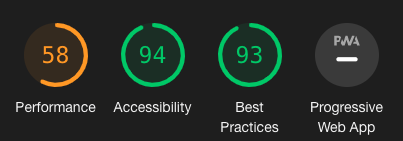
\includegraphics[width=0.5\textwidth]{10evaluation/images/lighthouse.png}
    \caption{Google Lighthouse scores for evaluation of the codeHelper application.}
    \label{fig:lighthouse}
\end{figure}

The aspects which most detriment performance are discussed in the limitations and future work section, \ref{sec:futurework}.

\newpage
\section{Comparing Existing Tools with codeHelper}

In this section, the existing tools analysed in Chapter \ref{chap:context} shall be compared to the developed codeHelper system.  

Table \ref{tab:comparetools} shows a side-by-side comparison of codeHelper, Spiceworks and ClassroomQ against the requirements outlined in chapter \ref{chap:req}. 

\begin{table}[H]
    \centering
    \begin{tabular}{c|c|c|c|c}
        & & codeHelper & Spiceworks & ClassroomQ \\
        \hline\hline
         F-01 & Users can Register & \color{green} \textbf{ \color{green} \textbf{\checked}} &  \color{green} \textbf{\checked} &  \color{green} \textbf{\checked} \\
         \hline
         F-02 & Users can Login with Shibboleth  & \color{red} \textbf{x}  & \color{red} \textbf{x}  & \color{red} \textbf{x} \\
         \hline
         F-03 & Admin can assign roles &  \color{green} \textbf{\checked} &  \color{green} \textbf{\checked}  & \color{red} \textbf{x} \\
         \hline
         F-04 & Users can Login/Logout &  \color{green} \textbf{\checked} &  \color{green} \textbf{\checked} &  \color{green} \textbf{\checked} \\
         \hline
         F-05 & Students can post tickets with info &  \color{green} \textbf{\checked} &  \color{green} \textbf{\checked}  & \color{red} \textbf{x} \\
          \hline
         F-06 & Students can add tags &  \color{green} \textbf{\checked}  & \color{red} \textbf{x}  & \color{red} \textbf{x} \\
          \hline
         F-07 & System recommends similar tickets  & \color{red} \textbf{x}  & \color{red} \textbf{x}  & \color{red} \textbf{x} \\
          \hline
         F-08 & Tracks selected ticket recommendation  & \color{red} \textbf{x}  & \color{red} \textbf{x}  & \color{red} \textbf{x} \\
          \hline
         F-09 & Demonstrator can assign self to ticket &  \color{green} \textbf{\checked} &  \color{green} \textbf{\checked}  & \color{red} \textbf{x} \\
          \hline
         F-10 & Demonstrator can chat on own tickets &  \color{green} \textbf{\checked}  & \color{red} \textbf{x}  & \color{red} \textbf{x} \\
          \hline
         F-11 & Demonstrator can close ticket &  \color{green} \textbf{\checked} &  \color{green} \textbf{\checked}  & \color{red} \textbf{x} \\
          \hline
         F-12 & Student can close ticket &  \color{green} \textbf{\checked}  & \color{red} \textbf{x}  & \color{red} \textbf{x} \\
          \hline
         F-13 & Lablead can open and close labs &  \color{green} \textbf{\checked}  & \color{red} \textbf{x}  & \color{red} \textbf{x} \\
          \hline
         F-14 & Lablead can disable accounts  & \color{red} \textbf{x}  & \color{red} \textbf{x}  & \color{red} \textbf{x} \\
          \hline
         F-15 & System prevents offensive content  & \color{red} \textbf{x}  & \color{red} \textbf{x}  & \color{red} \textbf{x} \\
          \hline
         F-16 & System allows users 1 live ticket &  \color{green} \textbf{\checked}  & \color{red} \textbf{x}  & \color{red} \textbf{x} \\
          \hline
         F-17 & Students can edit their live ticket  & \color{red} \textbf{x}  & \color{red} \textbf{x}  & \color{red} \textbf{x} \\
          \hline
         F-18 & Demonstrator can livechat on all tickets &  \color{green} \textbf{\checked}  & \color{red} \textbf{x}  & \color{red} \textbf{x} \\
        \hline
         F-19 & Users can video call &  \color{green} \textbf{\checked}  & \color{red} \textbf{x}  & \color{red} \textbf{x} \\
                 \hline
         F-20a & Demonstrator can create reusable solution &  \color{green} \textbf{\checked}  & \color{red} \textbf{x}  & \color{red} \textbf{x} \\
                 \hline
         F-20b & Demonstrator can edit existing solution &  \color{green} \textbf{\checked}  & \color{red} \textbf{x}  & \color{red} \textbf{x} \\
                 \hline
         F-20c & Demonstrator can assign solution to ticket &  \color{green} \textbf{\checked}  & \color{red} \textbf{x}  & \color{red} \textbf{x} \\
                 \hline
         F-21 & System prompts for solution to problems  & \color{red} \textbf{x}  & \color{red} \textbf{x}  & \color{red} \textbf{x} \\
                 \hline
         F-22 & Demonstrator can livechat on all tickets &  \color{green} \textbf{\checked}  & \color{red} \textbf{x} &  \color{green} \textbf{\checked} \\
                 \hline
         F-23 & User can specify in-person location &  \color{green} \textbf{\checked} &  \color{green} \textbf{\checked} &  \color{green} \textbf{\checked} \\
            \hline
         F-24 & User can send files &  \color{green} \textbf{\checked}  & \color{red} \textbf{x}  & \color{red} \textbf{x} \\
            \hline
         F-25 & System shows timeline of actions &  \color{green} \textbf{\checked} &  \color{green} \textbf{\checked}  & \color{red} \textbf{x} \\
            \hline
         F-26 & System shows statistics by lab &  \color{green} \textbf{\checked}  & \color{red} \textbf{x}  & \color{red} \textbf{x} \\
            \hline
          F-26 & System shows statistics by class &  \color{green} \textbf{\checked}  & \color{red} \textbf{x}  & \color{red} \textbf{x} \\
            \hline
    \end{tabular}
    \caption{Comparison of functional system requirements achieved by codeHelper, Spiceworks and ClassroomQ systems.}
    \label{tab:comparetools}
\end{table}



%
% Appendices
%
\appendix
%
% Thesis - Appendix A
% Jack McLean
% School of Computer Science
% University of St Andrews, Scotland, UK
% 2014
%



\chapter{Appendix-A Title}


%
% Thesis - Appendix A
% Jack McLean
% School of Computer Science
% University of St Andrews, Scotland, UK
% 2014
%



\chapter{Appendix-B Title}



%
% Glossary
%
\printglossaries

%
% Bibliography
%
\bibliographystyle{apalike}
\bibliography{thesis}

\end{document}
